\documentclass[oneside]{book}
\usepackage{xeCJK} % this is for Chinese
\usepackage{amsmath} % this is for math formatting and fonts
\usepackage{amssymb} % this is for math formatting and fonts
\usepackage{graphicx} % this is for including graphics
\usepackage{color} % this is for color
\usepackage{float} % this is for floating objects like tables and figures
\usepackage{caption} % this is for captions
\usepackage{subcaption} % this is for subcaptions
\usepackage{tikz} % this is for drawing figures
\usepackage{pgfplots} % this is for plotting data
\usepackage{algorithm} % this is for algorithms
\usepackage{algpseudocode} % this is for pseudocode
\usepackage{listings} % this is for typesetting code
\usepackage{booktabs} % this is for tables
\usepackage{multirow} % this is for tables
\usepackage{makeidx} % this is for creating indexes
\usepackage{lipsum} % this is for creating indexes
\usepackage{appendix} % this is for appendices
\usepackage{makecell} % this is for tables
\usepackage{longtable} % this is for tables
\usepackage{pdflscape} % this is for tables
\usepackage{rotating} % this is for tables
\usepackage{bm} % this is for bold math symbols
\usepackage{bbm} % this is for indicator function
\usepackage{setspace} % this is for line spacing
\usepackage{titlesec} % this is for section spacing
\usepackage{fancyhdr} % this is for headers and footers
\usepackage{pdfpages} % this is for including pdf files
\usepackage{enumitem} % this is for lists
\usepackage{natbib} % this is for references
\usepackage{bibentry} % this is for references
\usepackage{blindtext}
% 行间距 1.5 倍
\renewcommand{\baselinestretch}{1.5}
% 段前段后距离
\setlength{\parskip}{0.5\baselineskip}
% 段落缩进
\setlength{\parindent}{2em}
% 页边距 1.0cm
\usepackage{geometry}
\geometry{left=2.0cm,right=2.0cm,top=1.0cm,bottom=1.0cm}
% 页眉页脚,去掉页眉的那根横线
\pagestyle{fancy}
\renewcommand{\headrulewidth}{0pt}
% 页眉页脚,奇数页右,偶数页左
\fancyhead[RO,RE]{}
\fancyhead[LO,LE]{}
% 页码从正文开始计数
\setcounter{page}{1}
% 章节标题
\titleformat{\chapter}{\centering\Huge\bfseries}{}{1em}{}
\titleformat{\section}{\Large\bfseries}{\thesection}{1em}{}
\titleformat{\subsection}{\large\bfseries}{\thesubsection}{1em}{}
% 正文字体大小为 15pt, 行间距为 20pt
\defaultfontfeatures{Mapping=tex-text}
\setmainfont{Times New Roman}
\fontsize{18pt}{15pt}\selectfont
% section 和section* 的间距
% 图片和文字的间距
\titlespacing{\chapter} {5pt}{5pt}{5pt}
\titlespacing{\section} {5pt}{5pt}{5pt}
% 目录
\setcounter{tocdepth}{2}
% 代码
\lstset{language=Python}
\lstset{breaklines}
\lstset{extendedchars=false}
\lstset{numbers=left, numberstyle=\tiny, stepnumber=1, numbersep=5pt}
\lstset{frame=none,backgroundcolor=\color[RGB]{245,245,244}}
\lstset{keywordstyle=\color[RGB]{40,40,255}, 
        identifierstyle=\color[RGB]{0,0,0}, 
        numberstyle=\tiny\color[RGB]{0,192,192}, 
        commentstyle=\color[RGB]{0,96,96}, 
        stringstyle=\color[RGB]{128,0,0},
        showstringspaces=false,
        basicstyle=\ttfamily,
        breaklines=true}
% close page number
% \pagenumbering{gobble}
\begin{document}
\tableofcontents
\chapter{Similarity measure in neural networks}
\section*{Some comments}
This is just a personal note. It does not represent any company or group. 
If there are any errors, we can discuss them and welcome corrections. 
Different views can be discussed, and exchanges are welcome.

\section{Distance and similarity}
% 我觉得 similarity 这个概念是整个机器学习的核心。这个基本前提就是:相似的东西,应该离得近;离得近的东西,应该是相似的。
I think the concept of similarity is some what the core of machine learning. 
The basic premise is that \textcolor{red}{\textbf{similar things should be close, and things that are close should be similar.}}
% 最好的例子就是K-nearest-neighbor算法。这个算法的思想特别简单,如果一个人最好的10个朋友都经常去夜店,那么这个人大概率也经常去夜店。
The best example is the K-nearest-neighbor algorithm. If I am going to explain this algorithm in one sentence, I would say: 
\textbf{If a person's best 10 friends often go to nightclubs, then this person probably often goes to nightclubs.}
Let's consider three individuals:

\textbf{Person A} is from Wuhan, with a height of 179cm, weight of 70kg, aged 25. They enjoy playing basketball, work as a programmer, prefer using Taobao for shopping, and commute by bicycle.
\textbf{Person B}, also from Wuhan, is 180cm tall, weighs 70kg, aged 26. They share the same interests as Person A: playing basketball, working as a programmer, preferring Taobao for shopping, and commuting by bicycle.
\textbf{Person C}, from Shanghai, stands at 185cm, weighs 80kg, and is aged 54. Their hobbies include keeping up with the news, they work as an editor, prefer using JD (Jingdong) for shopping, and commute by car.

Further, we can represent these individuals' characteristics numerically. For instance, converting hobbies to numbers—playing basketball is 1, keeping up with the news is 2; converting occupations to numbers—programmer is 1, editor is 2; converting shopping platforms to numbers—Taobao is 1, JD is 2; and commuting methods to numbers—biking is 1, driving is 2.
Thus, we can represent these individuals' features in a tabular form:

\begin{table}[H]
        \centering
        \begin{tabular}{cccccccc}
        \hline
        height & weight & age & hobby & occupation & shopping & commute \\
        \hline
        179 & 70 & 25 & 1 & 1 & 1 & 1 \\
        180 & 70 & 26 & 1 & 1 & 1 & 1 \\
        185 & 80 & 54 & 2 & 2 & 2 & 2 \\
        \hline
        \end{tabular}
        \caption{Features}
\end{table}

This way, we've transformed people's characteristics into numerical representations, which is called \textbf{feature engineering}.
% 真实世界中,person A 和 person B 之间应该会更聊得来,因为他们有很多共同点。这意味着,A喜欢的东西,B也大概率会喜欢,那么推荐算法就可以推荐A喜欢的东西给B,反之亦然。
In the real world, Person A and Person B should get along well because they share many commonalities. This means that if A likes something, B will probably like it too. \textbf{Therefore, a recommendation algorithm can recommend things that A likes to B, and vice versa.}
Isn't sales volume determined in this way? If a person likes something, and their friends also like it, then the sales volume of that item will increase.

\textbf{To make it simple, similarity measure in mathematics is a distance measure.}
Different data types have different distance calculation methods. For example, cosine distance is often used to compare the similarity of two pieces of text.
% feature engineering对于传统的机器学习方法特别重要,feature engineering这一步主要通过人工来操作,如果特征工程做得不好,比如现实中A和B相似,但是向量B和向量A的距禰很远,甚至比向量C和向量A的距离还远,这样的话,机器学习的效果就会很差,因为数据质量低。
Feature engineering is particularly important for traditional machine learning methods. This step is mainly operated manually. If feature engineering is not done well, for example, if A and B are similar in reality, but the distance between vector A and vector B is very far, even farther than the distance between vector A and vector C, then the machine learning effect will be very poor because of low representation quality.

\section{Similarity in Binary Classification}
\subsection{Linear regression}
% regression可以简单理解为是一类找关系的task,寻找输入和输出之间的关系。
% 有一些输入和输出之间的关系是linear的,那么你用linear function去拟合这个关系,效果会很好。
Regression can be simply understood as a task of finding relationships, seeking the relationship between input and output. 
You have obersations $x_1,x_2,x_3,...,x_n$, and corresponding labels $y_1,y_2,y_3,...,y_n$. and you try to find a function $f(x)$, such that $f(x_i) \approx y_i$. 
Some relationships between input and output are linear. If you use a linear function to fit this relationship, the effect will be very good, otherwise, the effect will be poor.
\begin{figure}[H]
        \centering
        \includegraphics[width=0.4\textwidth]{images/linear regression.png}
        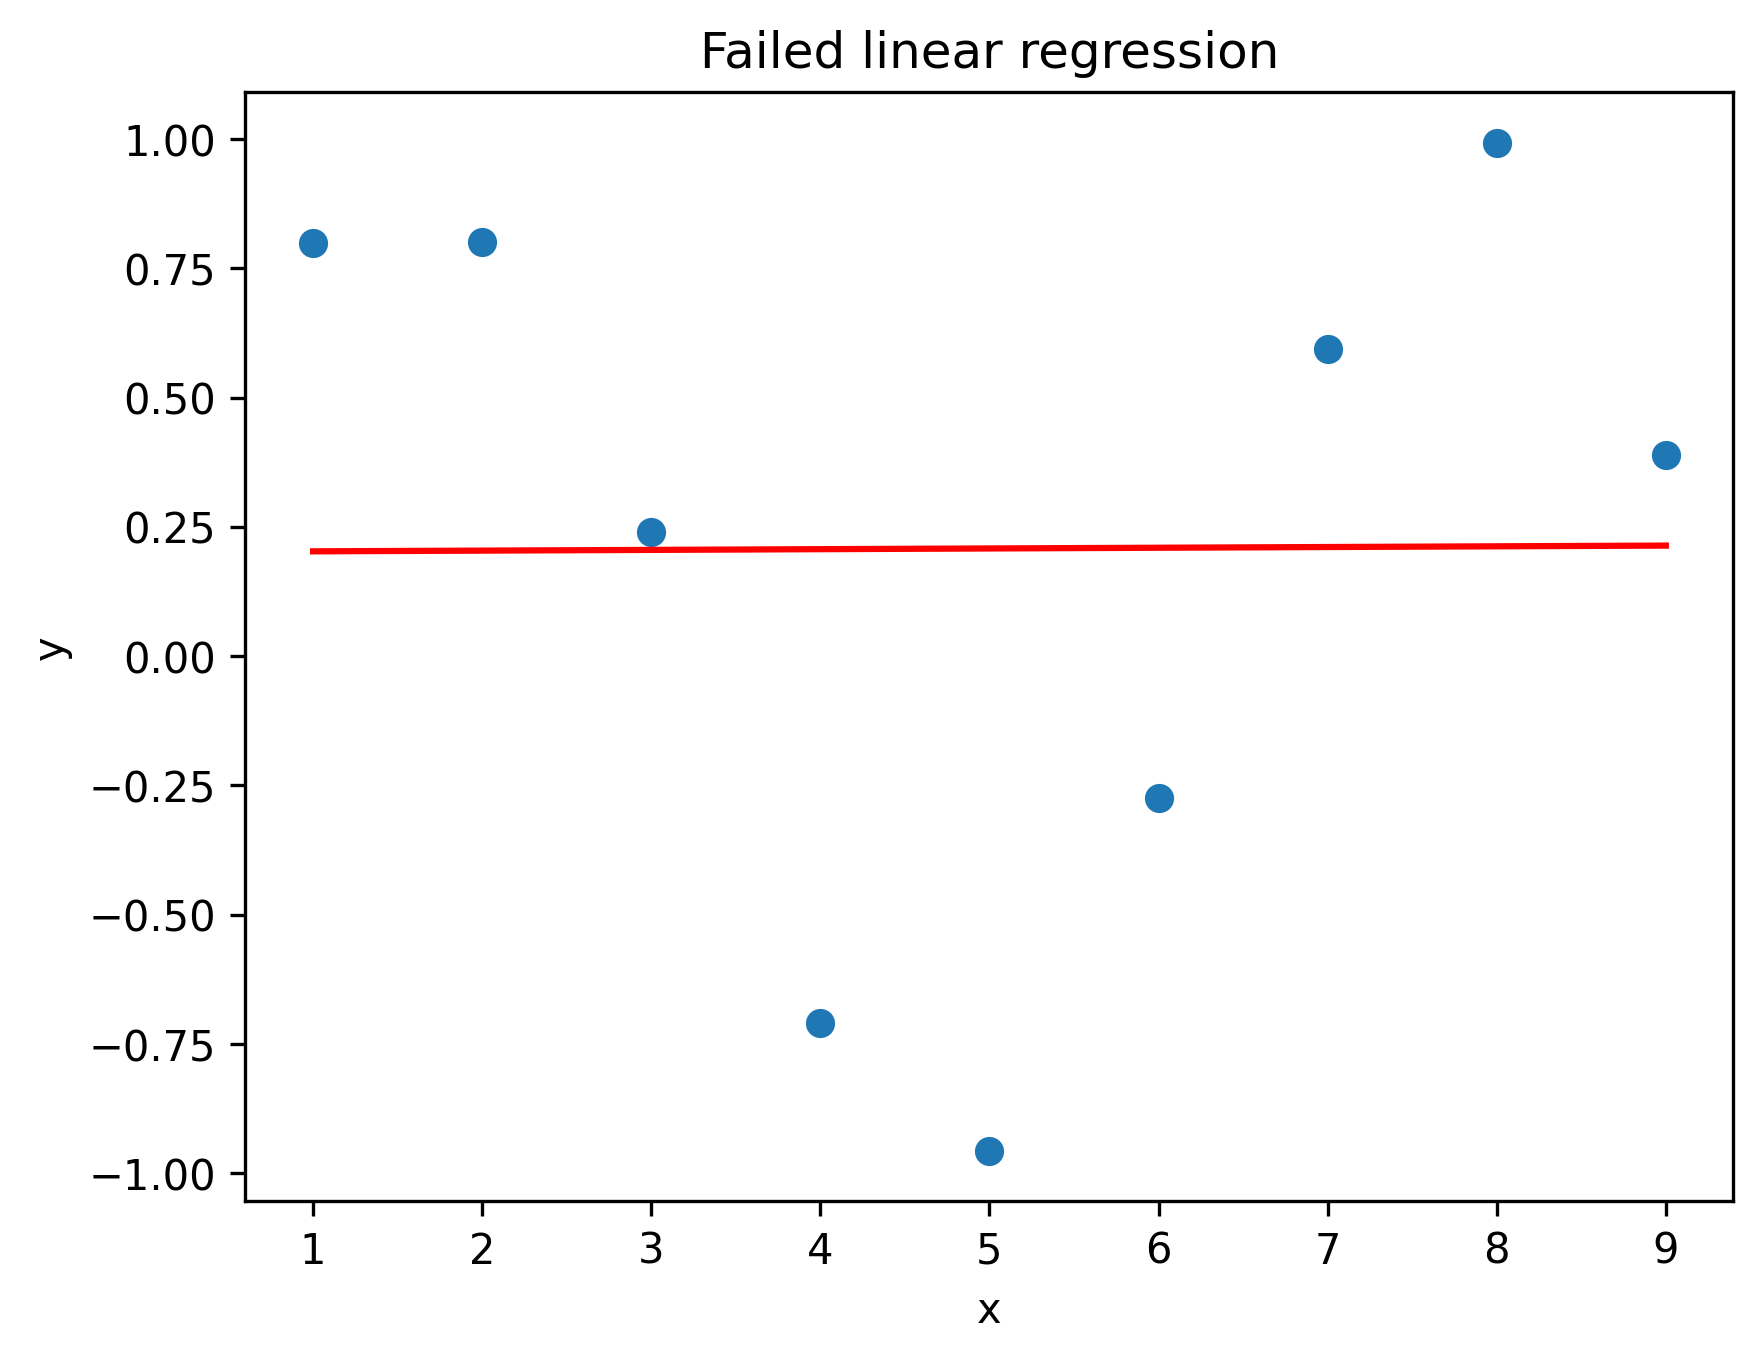
\includegraphics[width=0.43\textwidth]{images/failed linear regression.png}
        \caption{Linear regression}
        
\end{figure}
% 通常在regression task当中,我们会把y——true label和y_hat——predict label之间的差距定义为loss function,然后通过最小化loss function来找到最好的f(x)。
Usually, in the regression task, we define the difference between $y$ and $\hat{y}$ as the loss function, and then find the best $f(x)$ by minimizing the loss function.
\begin{figure}[H]
        \centering
        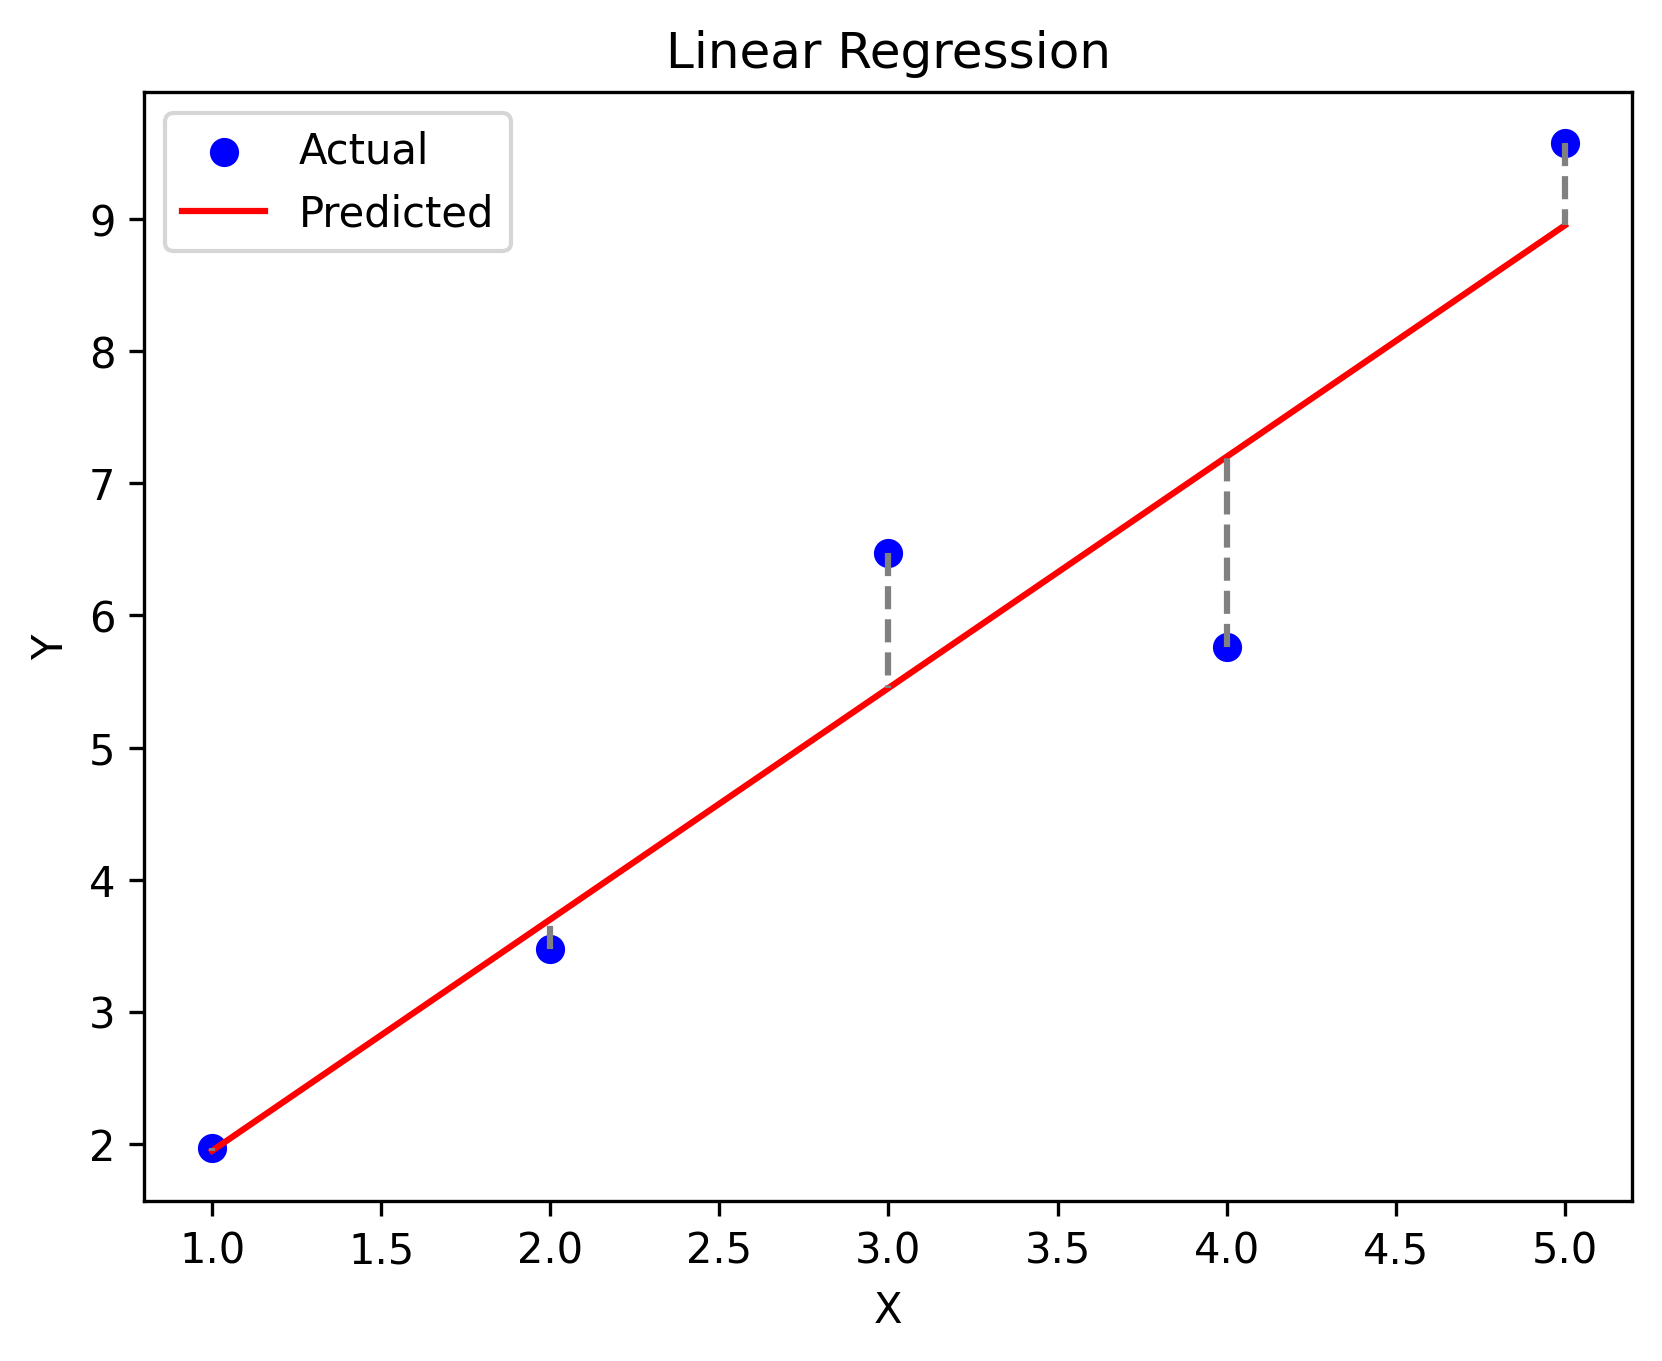
\includegraphics[width=0.5\textwidth]{images/y and predicted.png}
        \caption{Loss is the summation of the difference between y and predicted y}
        \label{fig:loss1}
\end{figure}
% I had a question before about why the loss function in linear regression is represented as a vertical line instead of the distance between the point and the line. **I think of linear regression as a tug-of-war game, where the points on either side of the line are pulling the line in opposite directions.**
\textcolor{blue}{\textbf{why the metric is not something like Figure \ref*{fig:loss2} instead of Figure \ref*{fig:loss1}?}}
why the loss function in linear regression is represented as a vertical line instead of the distance between the point and the line?

\begin{figure}[H]
        \centering
        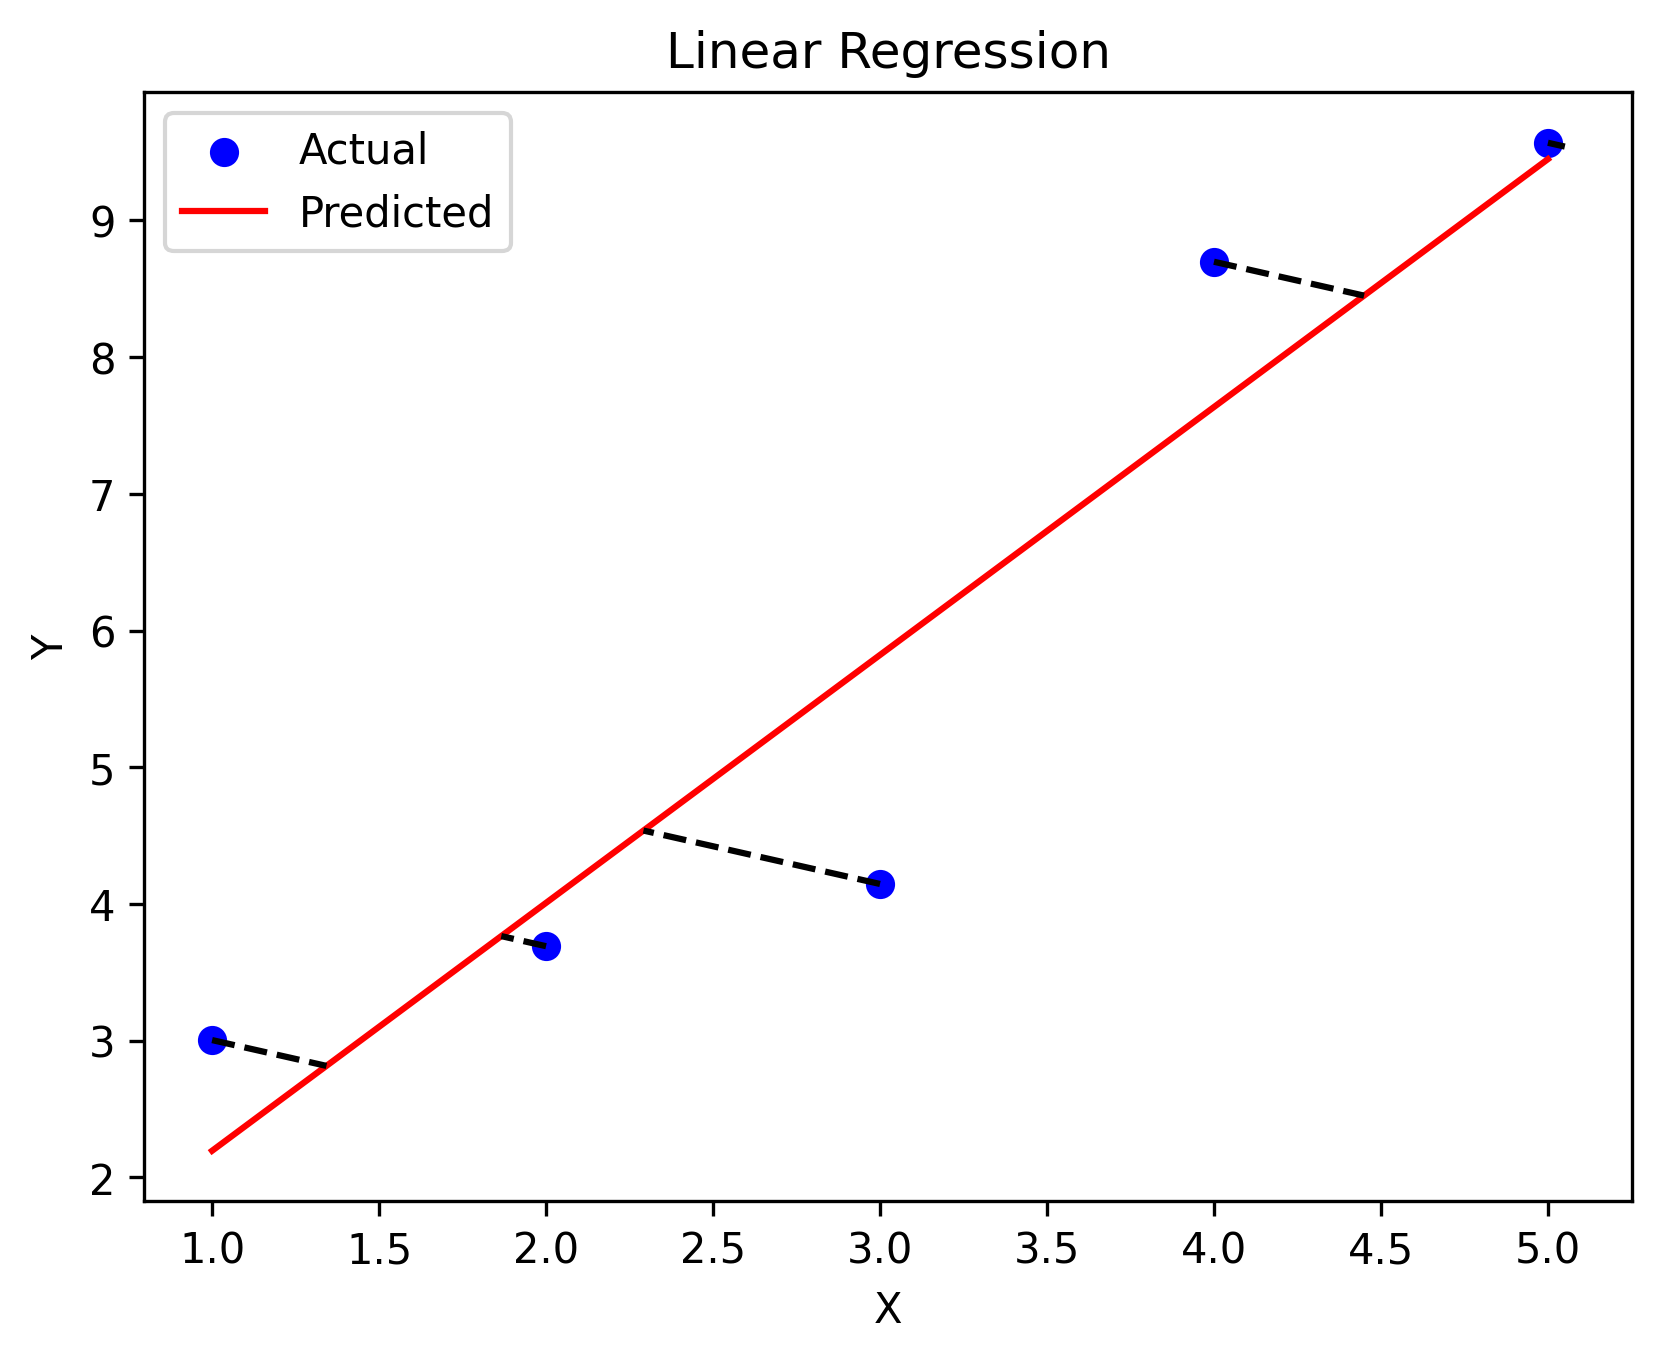
\includegraphics[width=0.5\textwidth]{images/Orthogonal lines.png}
        \caption{Distance: vertical and horizontal}
        \label{fig:loss2}
\end{figure}

my answer is \textcolor{blue}{we don't need both the horizontal and vertical distances, we only need the vertical distance.}  The vertical distance is the shift in the y-axis, this is what we care about.
\subsection{Logistic regression}
% 如果把线性回归的point,分成两类,一类是直线上方,一类是直线下方,那么这个问题就变成了一个binary classification的问题。
If we divide the points in linear regression into two categories, one above the line and one below the line, then this problem becomes a binary classification problem.
The line can be represented as $y = w_1x + w_0 = 0$, and the points above the line can be represented as $y = w_1x + w_0 > 0$, and the points below the line can be represented as $y = w_1x + w_0 < 0$.
\begin{equation}
        y = \begin{cases}
                Blue  & \text{if } w_1x + w_0 > 0 \\
                Yellow & \text{if } w_1x + w_0 < 0
        \end{cases}
        \label{eq:binary1}
\end{equation}
\begin{figure}[H]
        \centering
        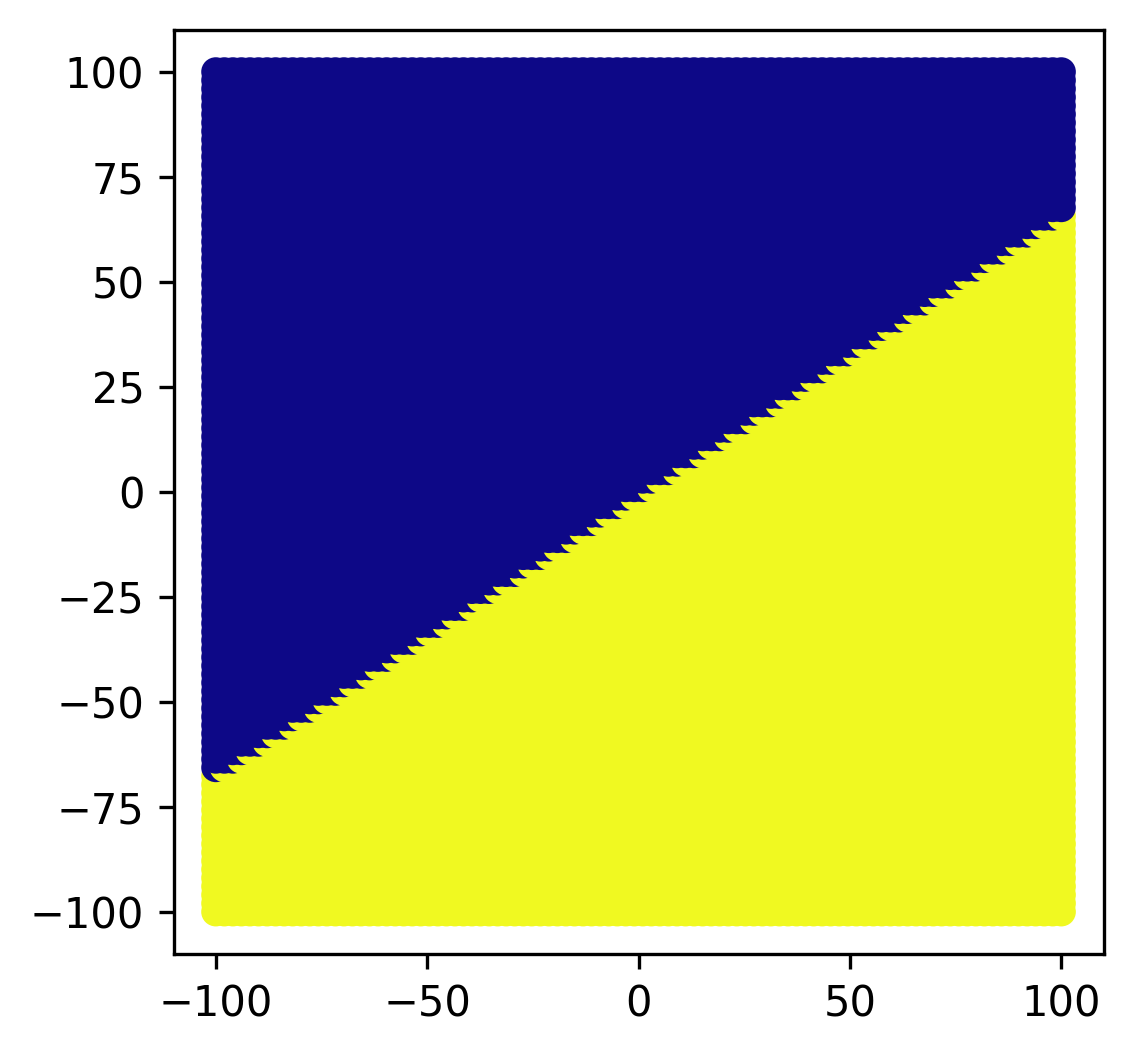
\includegraphics[width=0.5\textwidth]{images/binary class1.png}
        \caption{Binary classification}
        \label{fig:binary1}
\end{figure}

\textcolor{blue}{\textbf{Now we have a problem here: from Figure \ref{fig:binary1}, we don't know how far the point is from the line.}}
\textcolor{red}{\textbf{ We want to distinguish between the points that are close to the line and the points that are far from the line.}}
\begin{figure}[H]
        \centering
        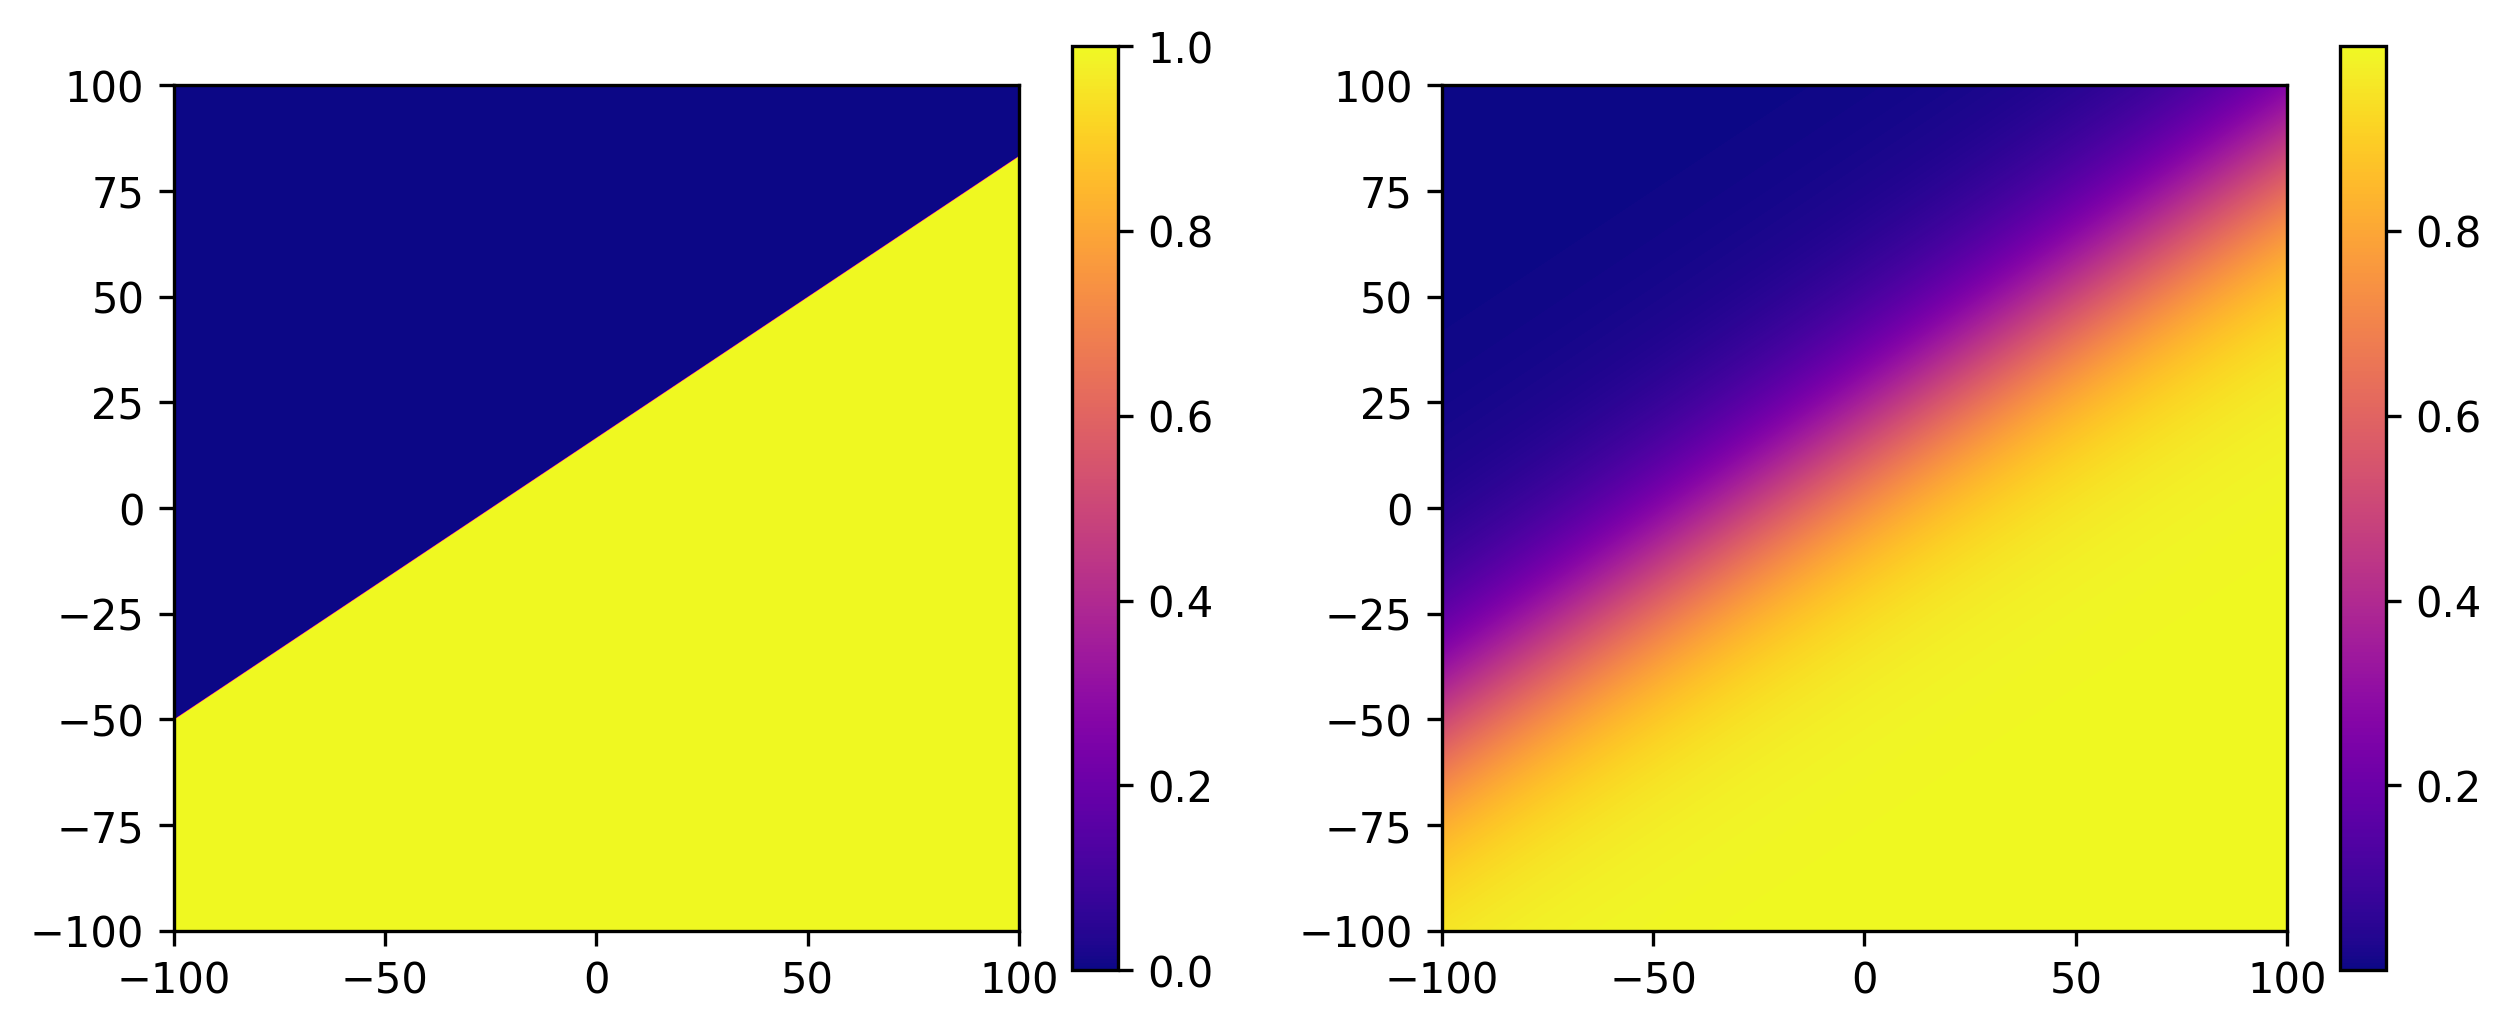
\includegraphics[width=1.0\textwidth]{images/binaryclass2.png}
        \caption{Binary classification}
        \label{fig:binary2}
\end{figure}
\begin{equation}
        \sigma (z) = \frac{1}{1+e^{-z}}
        \label{eq:binary2}
\end{equation}

% 为了解决这个问题,我们可以把线性回归的结果,通过一个sigmoid函数,把结果转换成0到1之间的值,这个值可以理解为是这个点离直线的距离。
To solve this problem, we can take the result of linear regression and convert it into a value between 0 and 1 using a sigmoid function. 
This value can be understood as the distance of the point from the line.
% 离直线越远,这个值越接近0 或者 1,离直线越近,这个值越接近0.5。
The farther the point is from the line, the closer this value is to 0 or 1, and the closer the point is to the line, the closer this value is to 0.5.
% 现在我们来看一个实际的例子。

Now let's look at an actual example.
% % 假设我现在已经把猫的特征(ear shape,nose size)和狗的特征都转换成了$N$维向量,我们的目标是对猫和狗做区分。

Suppose we have already converted the features of cats (ear shape, nose size) and dogs (ear shape, nose size) into $2$-dimensional vectors. Our goal is to distinguish between cats and dogs.
\begin{figure}[H]
        \centering
        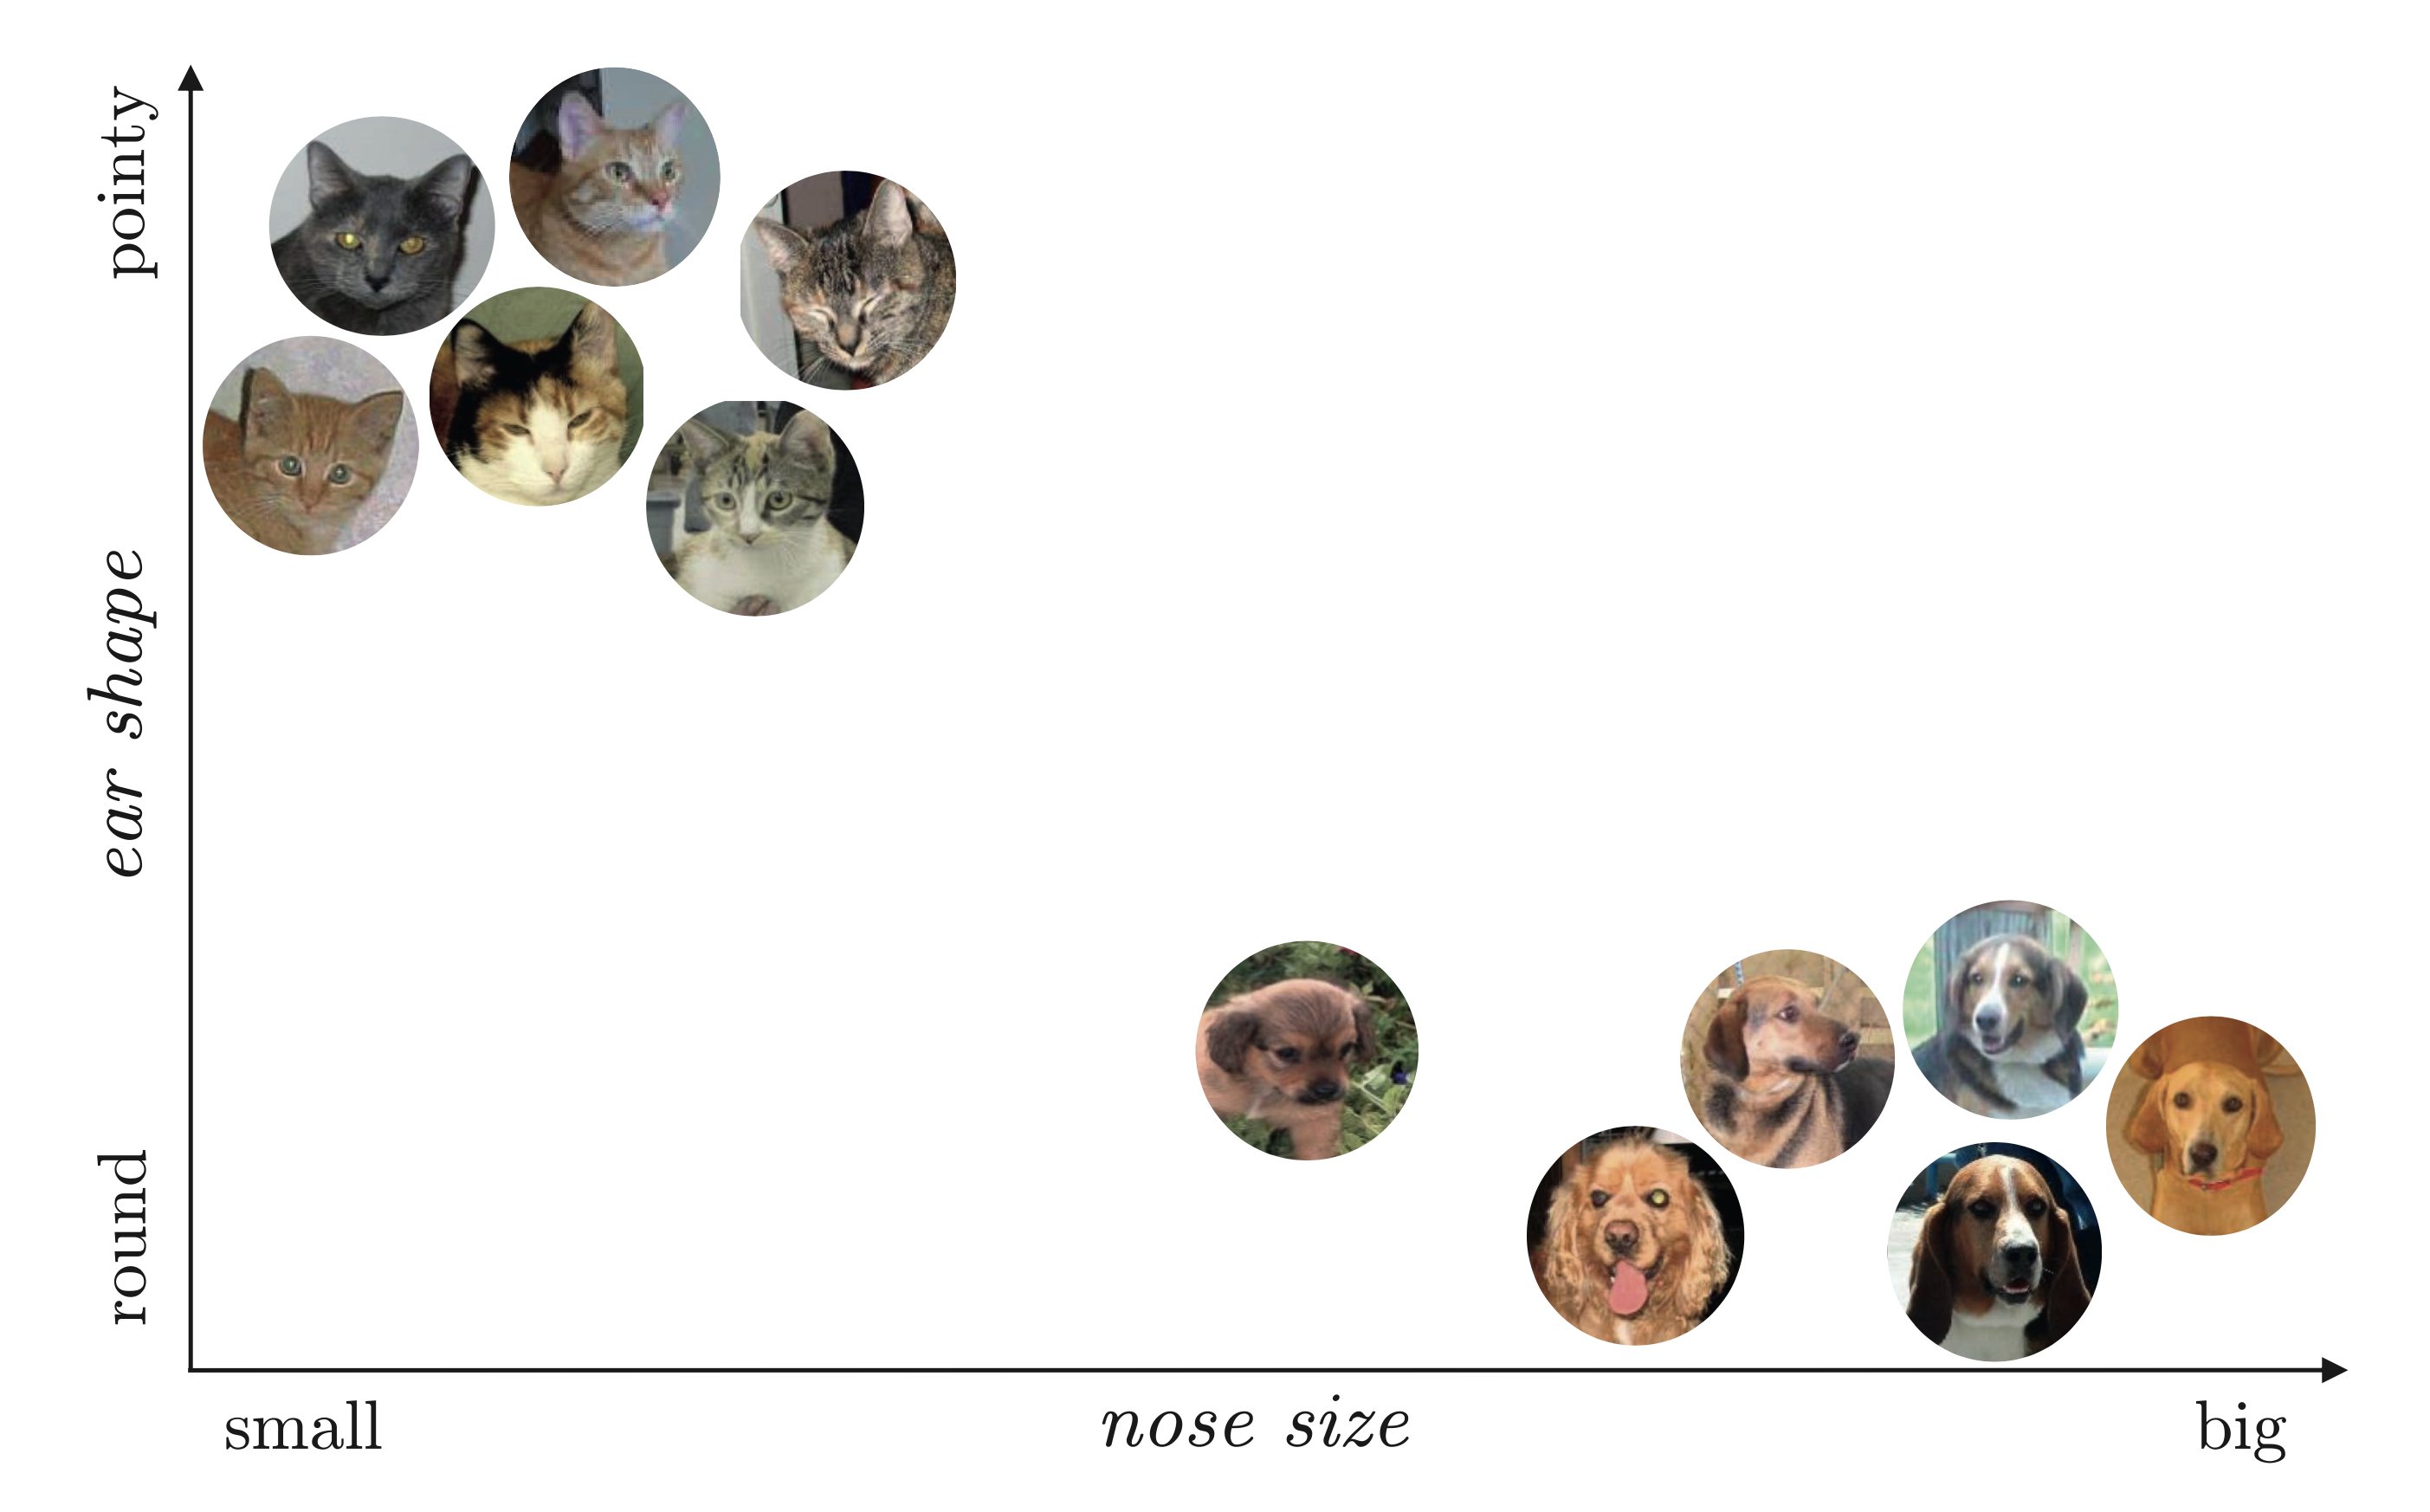
\includegraphics[width=0.5\textwidth]{images/feature embedding.png}
        \caption{Cat and Dog}
        \caption*{Image source: BOOK machine learning refined}
\end{figure}
% 我们需要找一根线,这根线可以把猫和狗分开, 这样的线就是我们的decision boundary。
We need to find a line that can separate cats and dogs. This line is our decision boundary.
\begin{figure}[H]
        \centering
        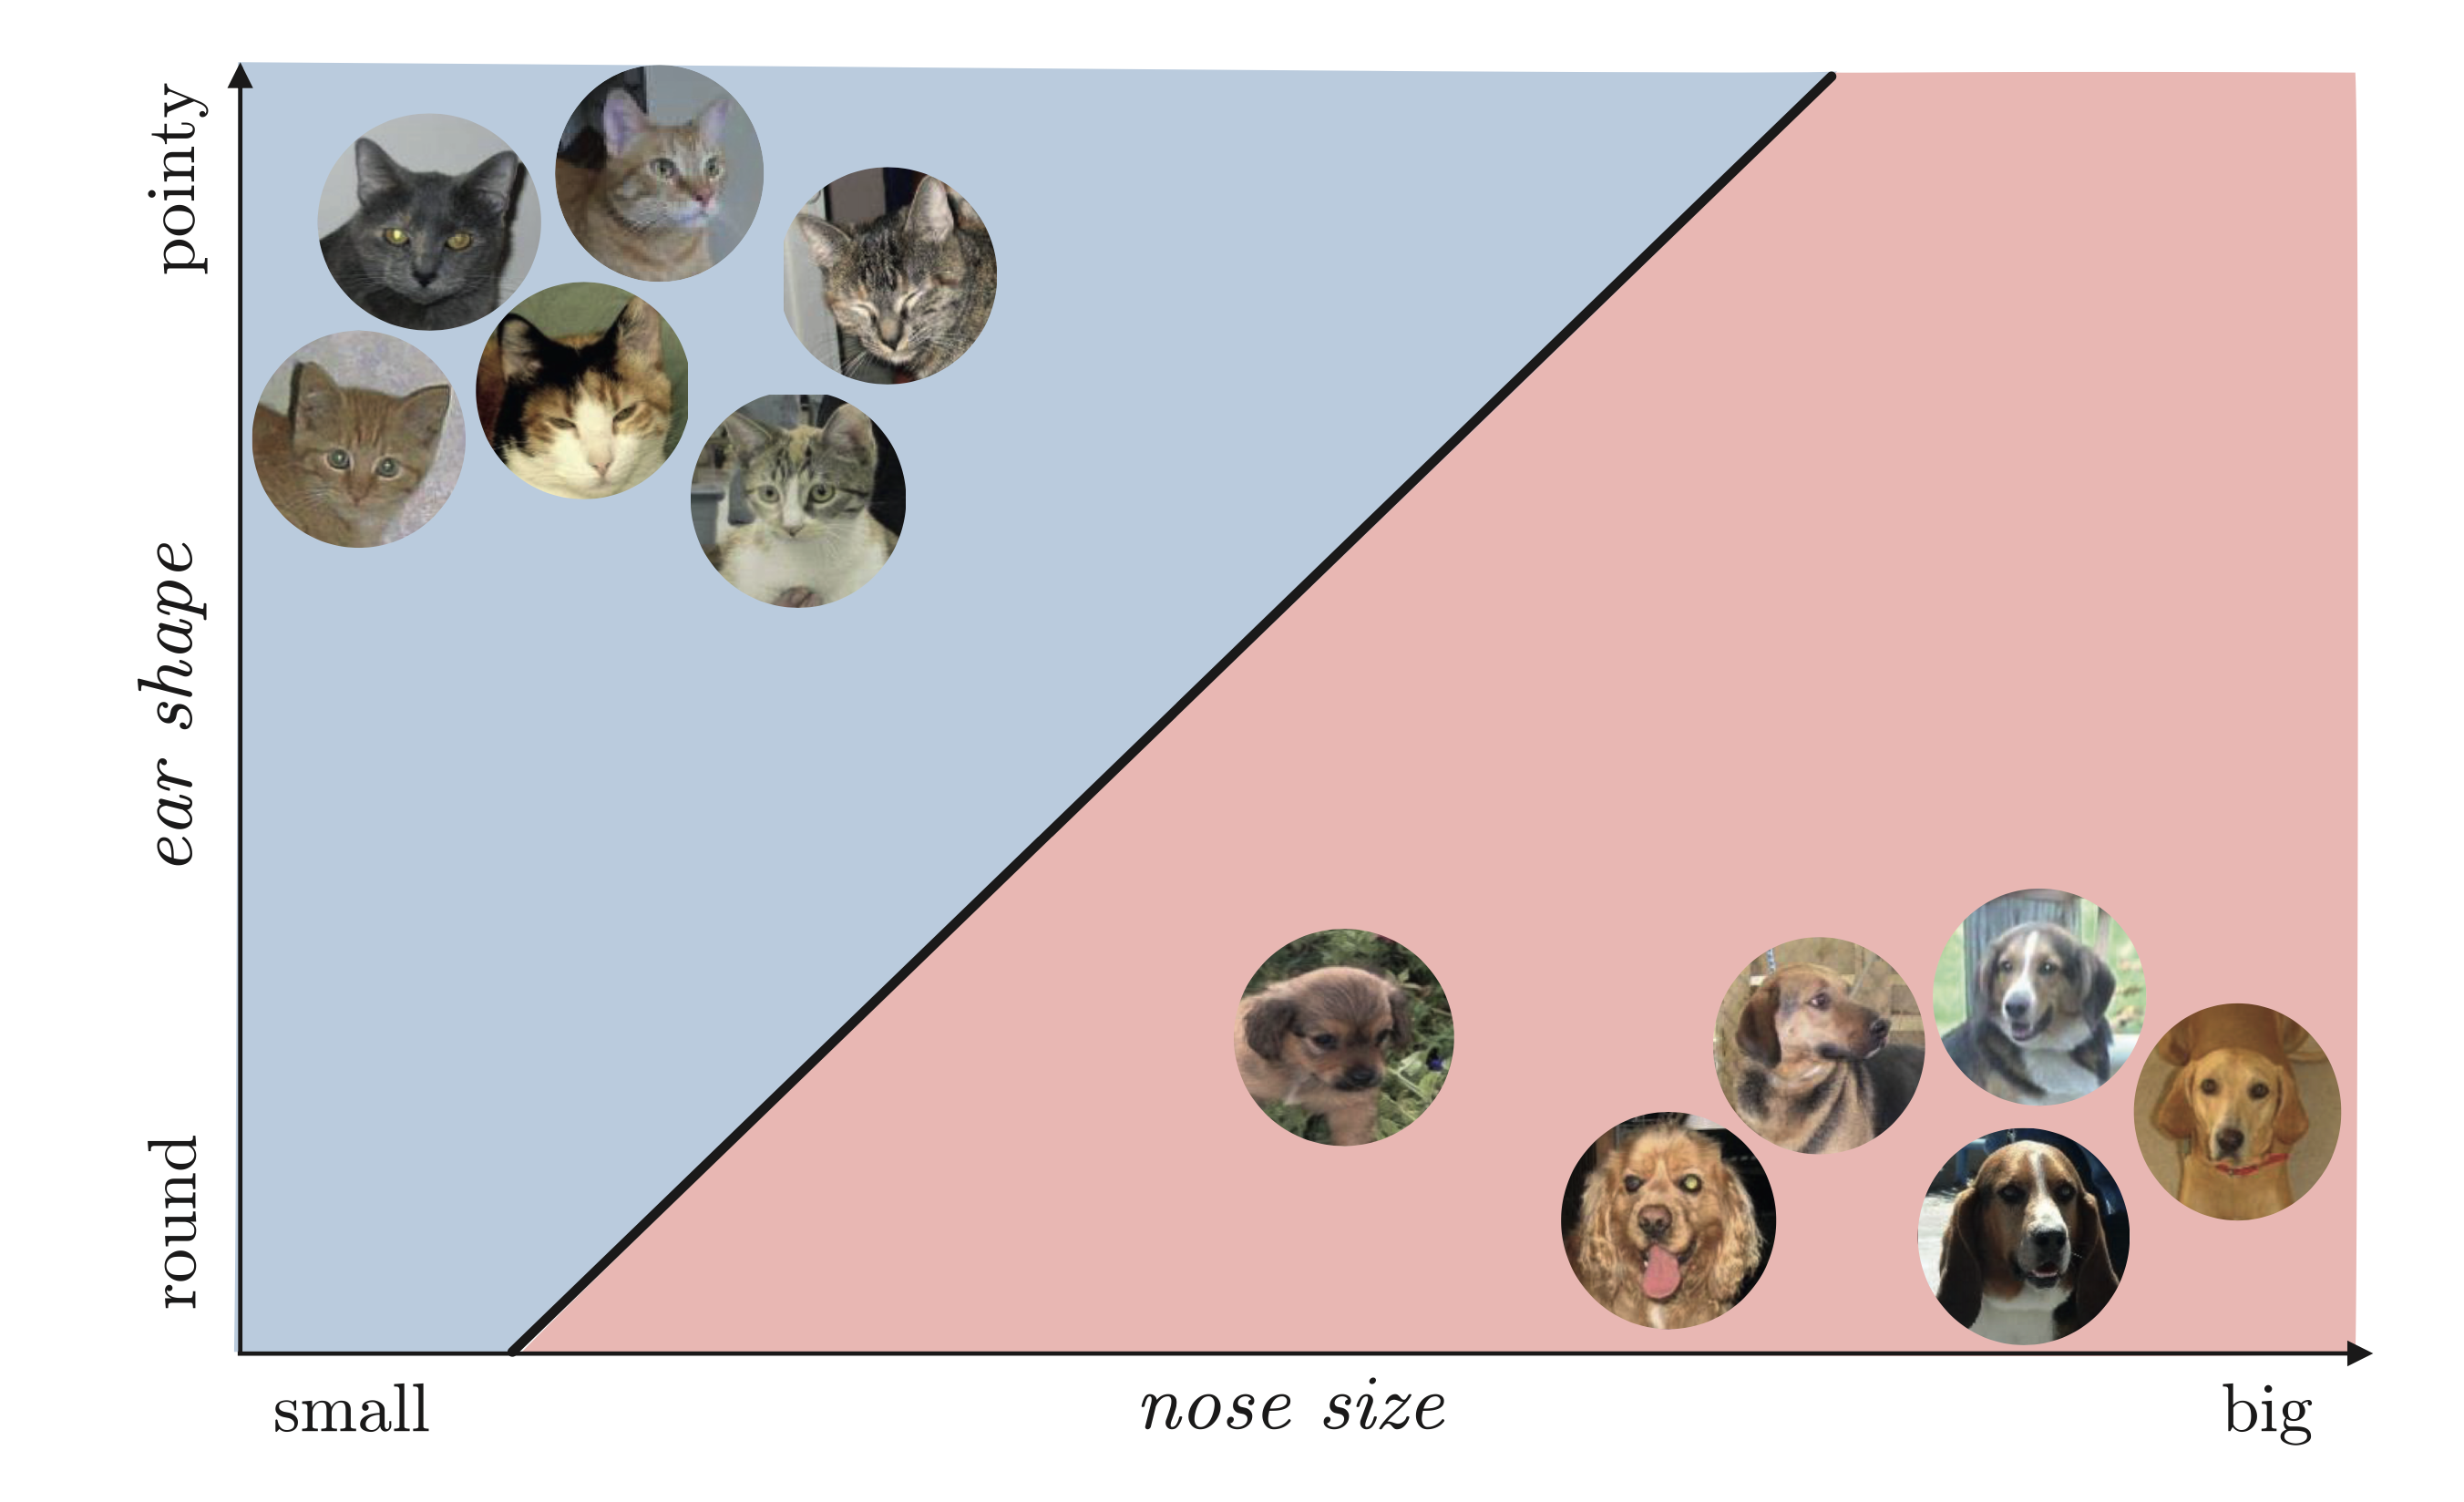
\includegraphics[width=0.6\textwidth]{images/decision boundary.png}
        \caption{Decision boundary}
        \caption*{Image source: BOOK machine learning refined}
\end{figure}

% 这句话可能有一些绕口,但是我想你会明白的,有一些猫比另外一些猫更像猫。
This sentence may be a bit convoluted, but I think you will understand. Some cats are more like cats than other cats.
% 有一些女性具有典型的女性外貌特征,有一些男性具有典型的男性外貌特征,但是也有一些人比较中性化。
For example, some women have typical “female” facial,some men have typical “male” facial features, but some people are more androgynous.
% 在decesion boundary附近的这些动物,可能是一些中性化的动物,他们的特征既有猫的特征,也有狗的特征。
The animals near the decision boundary may be androgynous animals. They have both cat-like and dog-like features.
% 越是远离decision boundary的动物,他们的特征就越明显,他们要么是典型的猫,要么是典型的狗。
The farther away from the decision boundary, the more obvious their features are. 
% 另外值得一提的是,sigmoid的输出是0到1之间的值,比如0.3,这意味着,也许有30%猫的特征,70%狗的特征。

It is worth mentioning that the output of the sigmoid is a value between 0 and 1, such as 0.3. This means that perhaps 30\% of the features are cat-like and 70\% are dog-like.
% 说明这可能是一只狗。
This indicates that this may be a dog.Plus, the decision boundary is not necessarily a straight line. It can be a curve, a circle, or any shape.

\subsection{Some other Classification methods}
\begin{figure}[H]
        \centering
        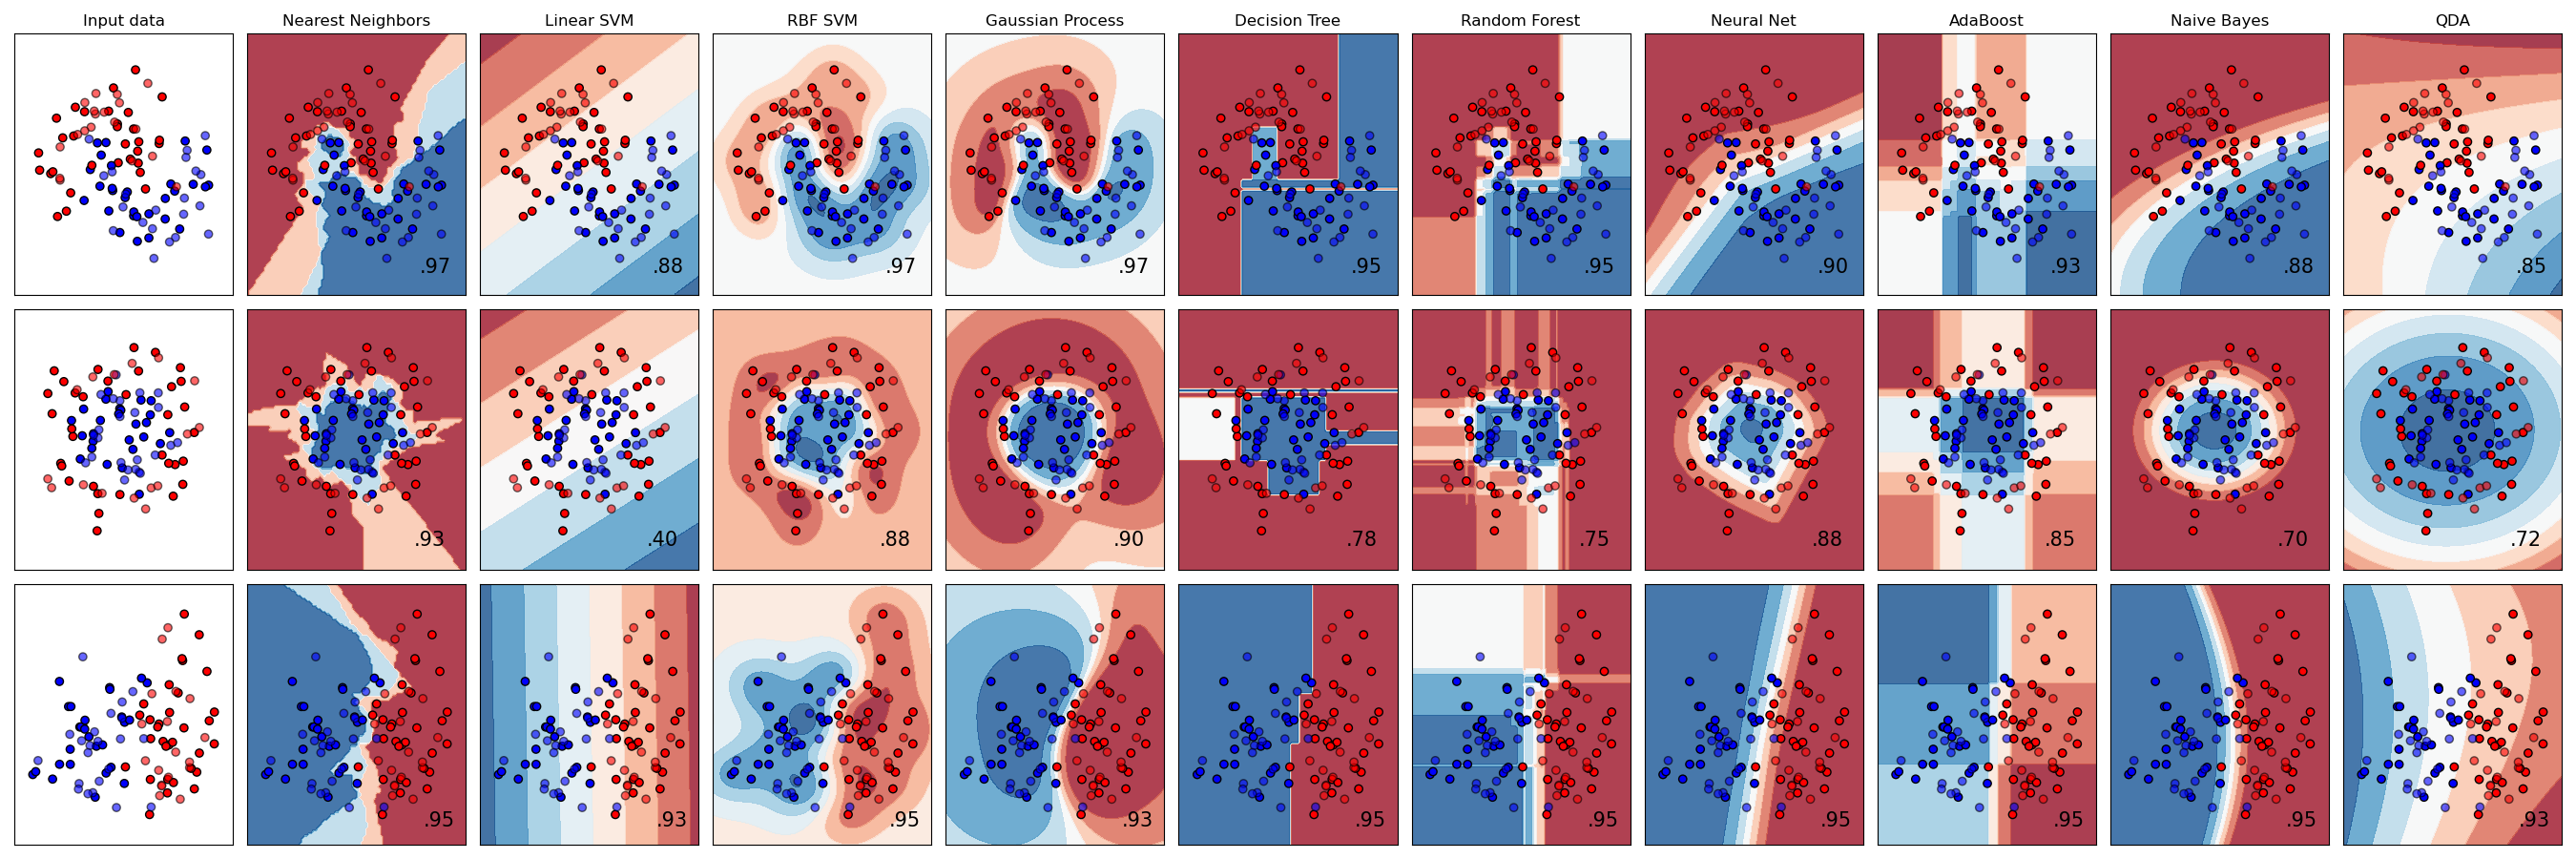
\includegraphics[width=0.9\textwidth]{images/classifier.png}
        \caption{Decision boundary by different classifiers}
        \caption*{Image source: scikit-learn classifier comparison}
\end{figure}


% 传统机器学习方法中,有很多分类器,比如SVM,KNN,Decision Tree,Random Forest等等,这些分类器能制造的decision boundary是不一样的,并且分类的效果高度依赖数据的分布。
In traditional machine learning methods, there are many classifiers, such as SVM, KNN, Decision Tree, Random Forest, etc. 
The decision boundaries that these classifiers can create are different, and the classification performance depends highly on the distribution of the data.
% 你可以把这些分类器都看成是函数approximator,他们的目标都是找到一个合适的boundary,这个boundary可以把不同类别的数据分开。
% 但是这些fucntion approximator的能力是有限的,他们只适合特定的一些数据,也就是说,他们不是通用的。
You can think of these classifiers as \textbf{function approximators}. Their goal is to find a suitable boundary that can separate data of different classes.
However, the ability of these function approximators is limited. They are only suitable for specific data, meaning they are \textbf{not universal}.
% 这些传统机器学习算法的设计需要一些数学基础,比如凸优化,概率论,线性代数等等。我觉得这些算法背后的思想是很值得学习的。
The design of these traditional machine learning algorithms requires some mathematical foundation, such as convex optimization, probability theory, linear algebra, etc. I think the ideas behind these algorithms are worth learning.

\section{Similarity in Covlutional Neural Networks(CNN)}
% CNN 里面包括Convolutional layer,Pooling layer,Fully connected layer。 Convolutional layer的作用是提取特征,Pooling layer的作用是降维,Fully connected layer的作用是分类。
CNN includes Convolutional layer, Pooling layer, Fully connected layer. The Convolutional layer extracts features, the Pooling layer reduces dimensionality, and the Fully connected layer classifies.
% 我只打算在这里讲一下Convolutional layer,我认为这是CNN里面最重要的一部分。
I only plan to talk about the Convolutional layer here, which I think is the most important part of CNN.
% https://ww2.mathworks.cn/help/deeplearning/ug/introduction-to-convolutional-neural-networks.html
\begin{figure}[H]
        \centering
        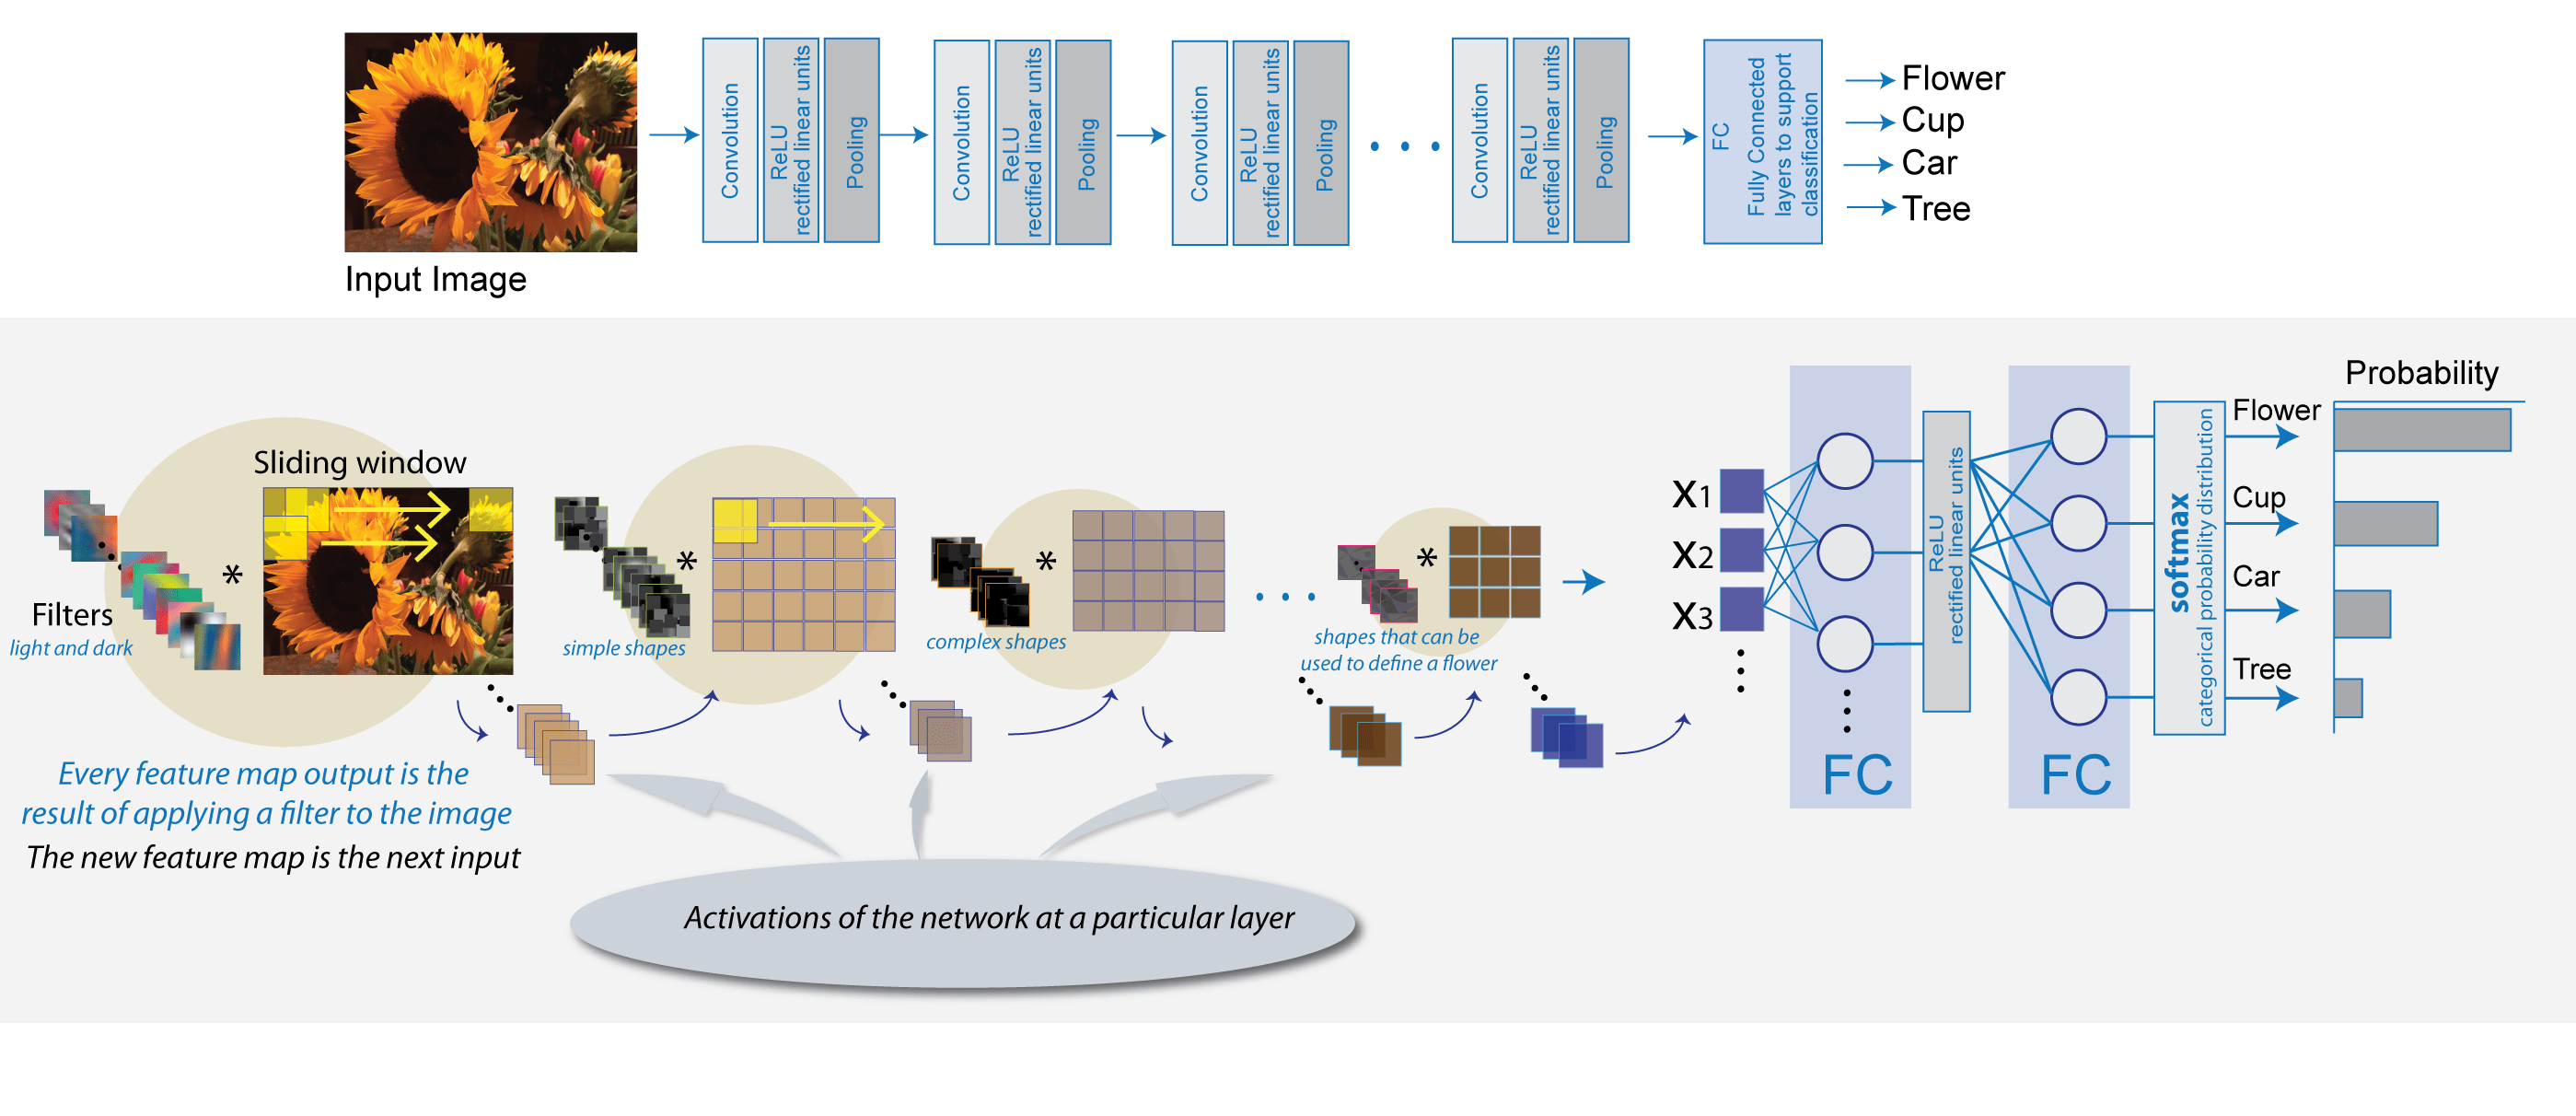
\includegraphics[width=1.0\textwidth]{images/CNN.png}
        \caption{CNN}
        \caption*{Image source: MathWorks introduction-to-convolutional-neural-networks}
\end{figure}
\begin{figure}[H]
        \centering
        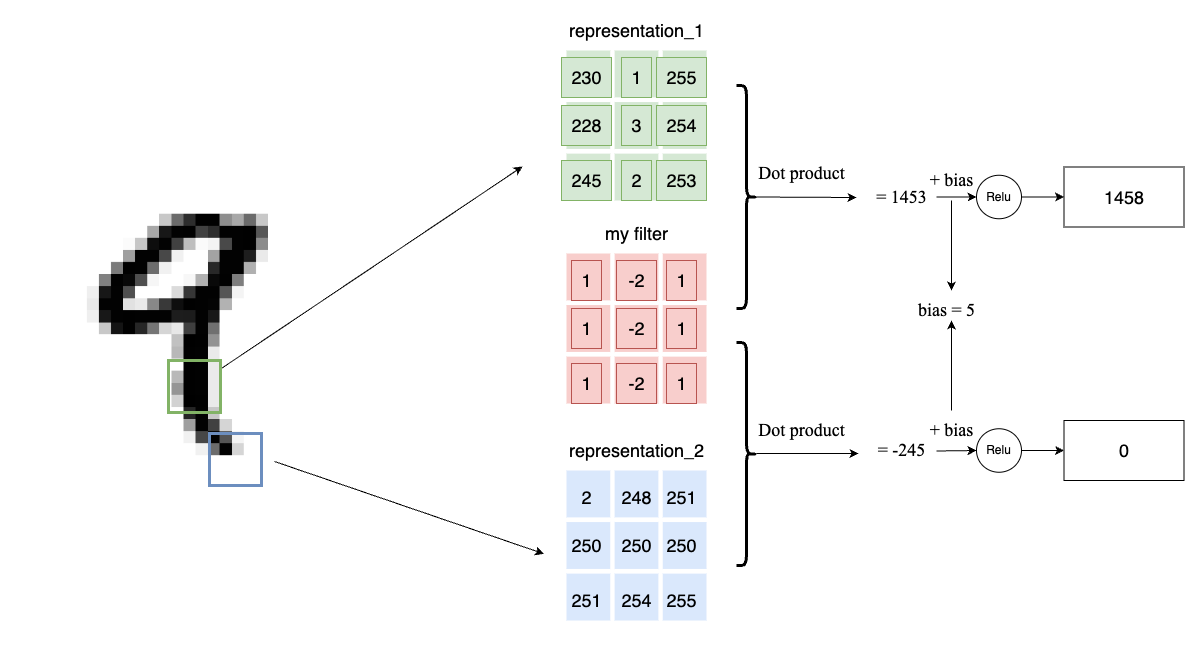
\includegraphics[width=0.9\textwidth]{images/CNN_si.png}
        \caption{Dot product and similarity}
\end{figure}

The process of the Convolutional layer is to calculate the \textcolor{red}{dot product} between the filter and the image representation, then add the bias, and then pass through an activation function, such as ReLU, and finally output a feature map. 
% 这个操作的关键在于,如果一个image representation和一个filter的dot product很大,那么这个image representation和这个filter是相似的。
\textbf{\textcolor{blue}{The key to this operation is that if the \textcolor{red}{dot product} between an image representation and a filter is large, then this image representation and this filter are similar. Conversely, if the numerical value after convolution is very small, then this image representation and this filter are dissimilar.}} 
% 我觉得Max pooling的作用进一步强调了这一点,Max pooling的作用是找到一个filter里面最大的值,也就是选择最相似的那个值。
I think the role of Max pooling further emphasizes this point. The role of Max pooling is to find the largest value in a filter, that is, to select the most similar value.

\section{Similarity in Deep Neural Networks(DNN)}
% 我觉得CNN就是DNN的一个特殊例子。
I think CNN is a special case of DNN.
% CNN 的参数更少一些,但是本质就是个DNN。
CNN has fewer parameters, but it is essentially a DNN.

% 对于 28 × 28 × 1 的输入图像,如果下一个隐藏层的神经元数量为 28 × 28 × 1 个 (图像大小不变)且采用全连接,那么将有 28 × 28 × 1 × 28 × 28 × 1 = 614656 个权值参数。
For a 28 × 28 × 1 input image, if the number of neurons in the next hidden layer is 28 × 28 × 1 (the image size remains unchanged) and fully connected, then there will be 28 × 28 × 1 × 28 × 28 × 1 = 614656 weight parameters.
% 采用 3 × 3 卷积,可以理解 成隐藏层的每个神经元只与输入层的 9 个神经元相连,其他连接都被剪枝,并且,各个位置 的连接参数是共享的,即只需要 9 个参数就可以完成任务。
Using a 3 × 3 convolution, it can be understood that each neuron in the hidden layer is only connected to 9 neurons in the input layer, and other connections are pruned. 
% 参数,subset
\textbf{Isn't this a subset of the fully connected layer?}
\begin{figure}[H]
        \centering
        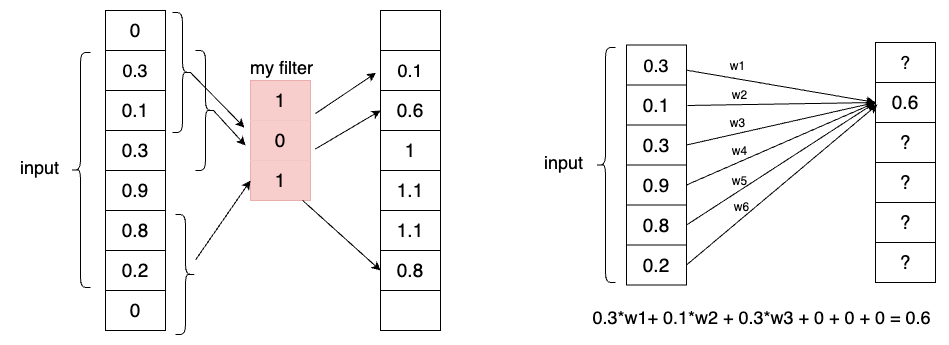
\includegraphics[width=1.0\textwidth]{images/CNN and DNN.png}
        \caption{CNN and DNN}
\end{figure}
% CNN 用了一种非常巧妙的方法,有效的降低了DNN的参数。
CNN uses a very clever method to effectively reduce the parameters of DNN.
% 我想说的是,DNN也是存在similarity measure,和 CNN 一样,或者事实上可以达到和CNN一样的效果,只要给的层数足够多。
What I want to say is that DNN also has a similarity measure, just like CNN, or in fact, it can achieve the same effect as CNN as long as the number of layers is sufficient.
\section{Similarity in Attention Mechanism}
Attention has 3 components: query, key, and value. 
Simply put, $Q$ and $K$ do \textcolor{red}{dot product}, then let it go through softmax, then multiply by $V$, and output. How you design $K, V$, and $Q$ depends on your task. $d_k$ is the dimension of $K$, $\frac{1}{\sqrt{d_k}}$ is to prevent the value of $Q K^T$ from being too large.
\begin{equation}
        \operatorname{Attention}(K, V, Q)=\operatorname{softmax}\left(\frac{Q K^T}{\sqrt{d_k}}\right) V
\end{equation}
\textbf{\textcolor{blue}{The \textcolor{red}{dot product} of $Q$ and $K^T$ is the similarity measure.}}
\begin{figure}[H]
        \centering
        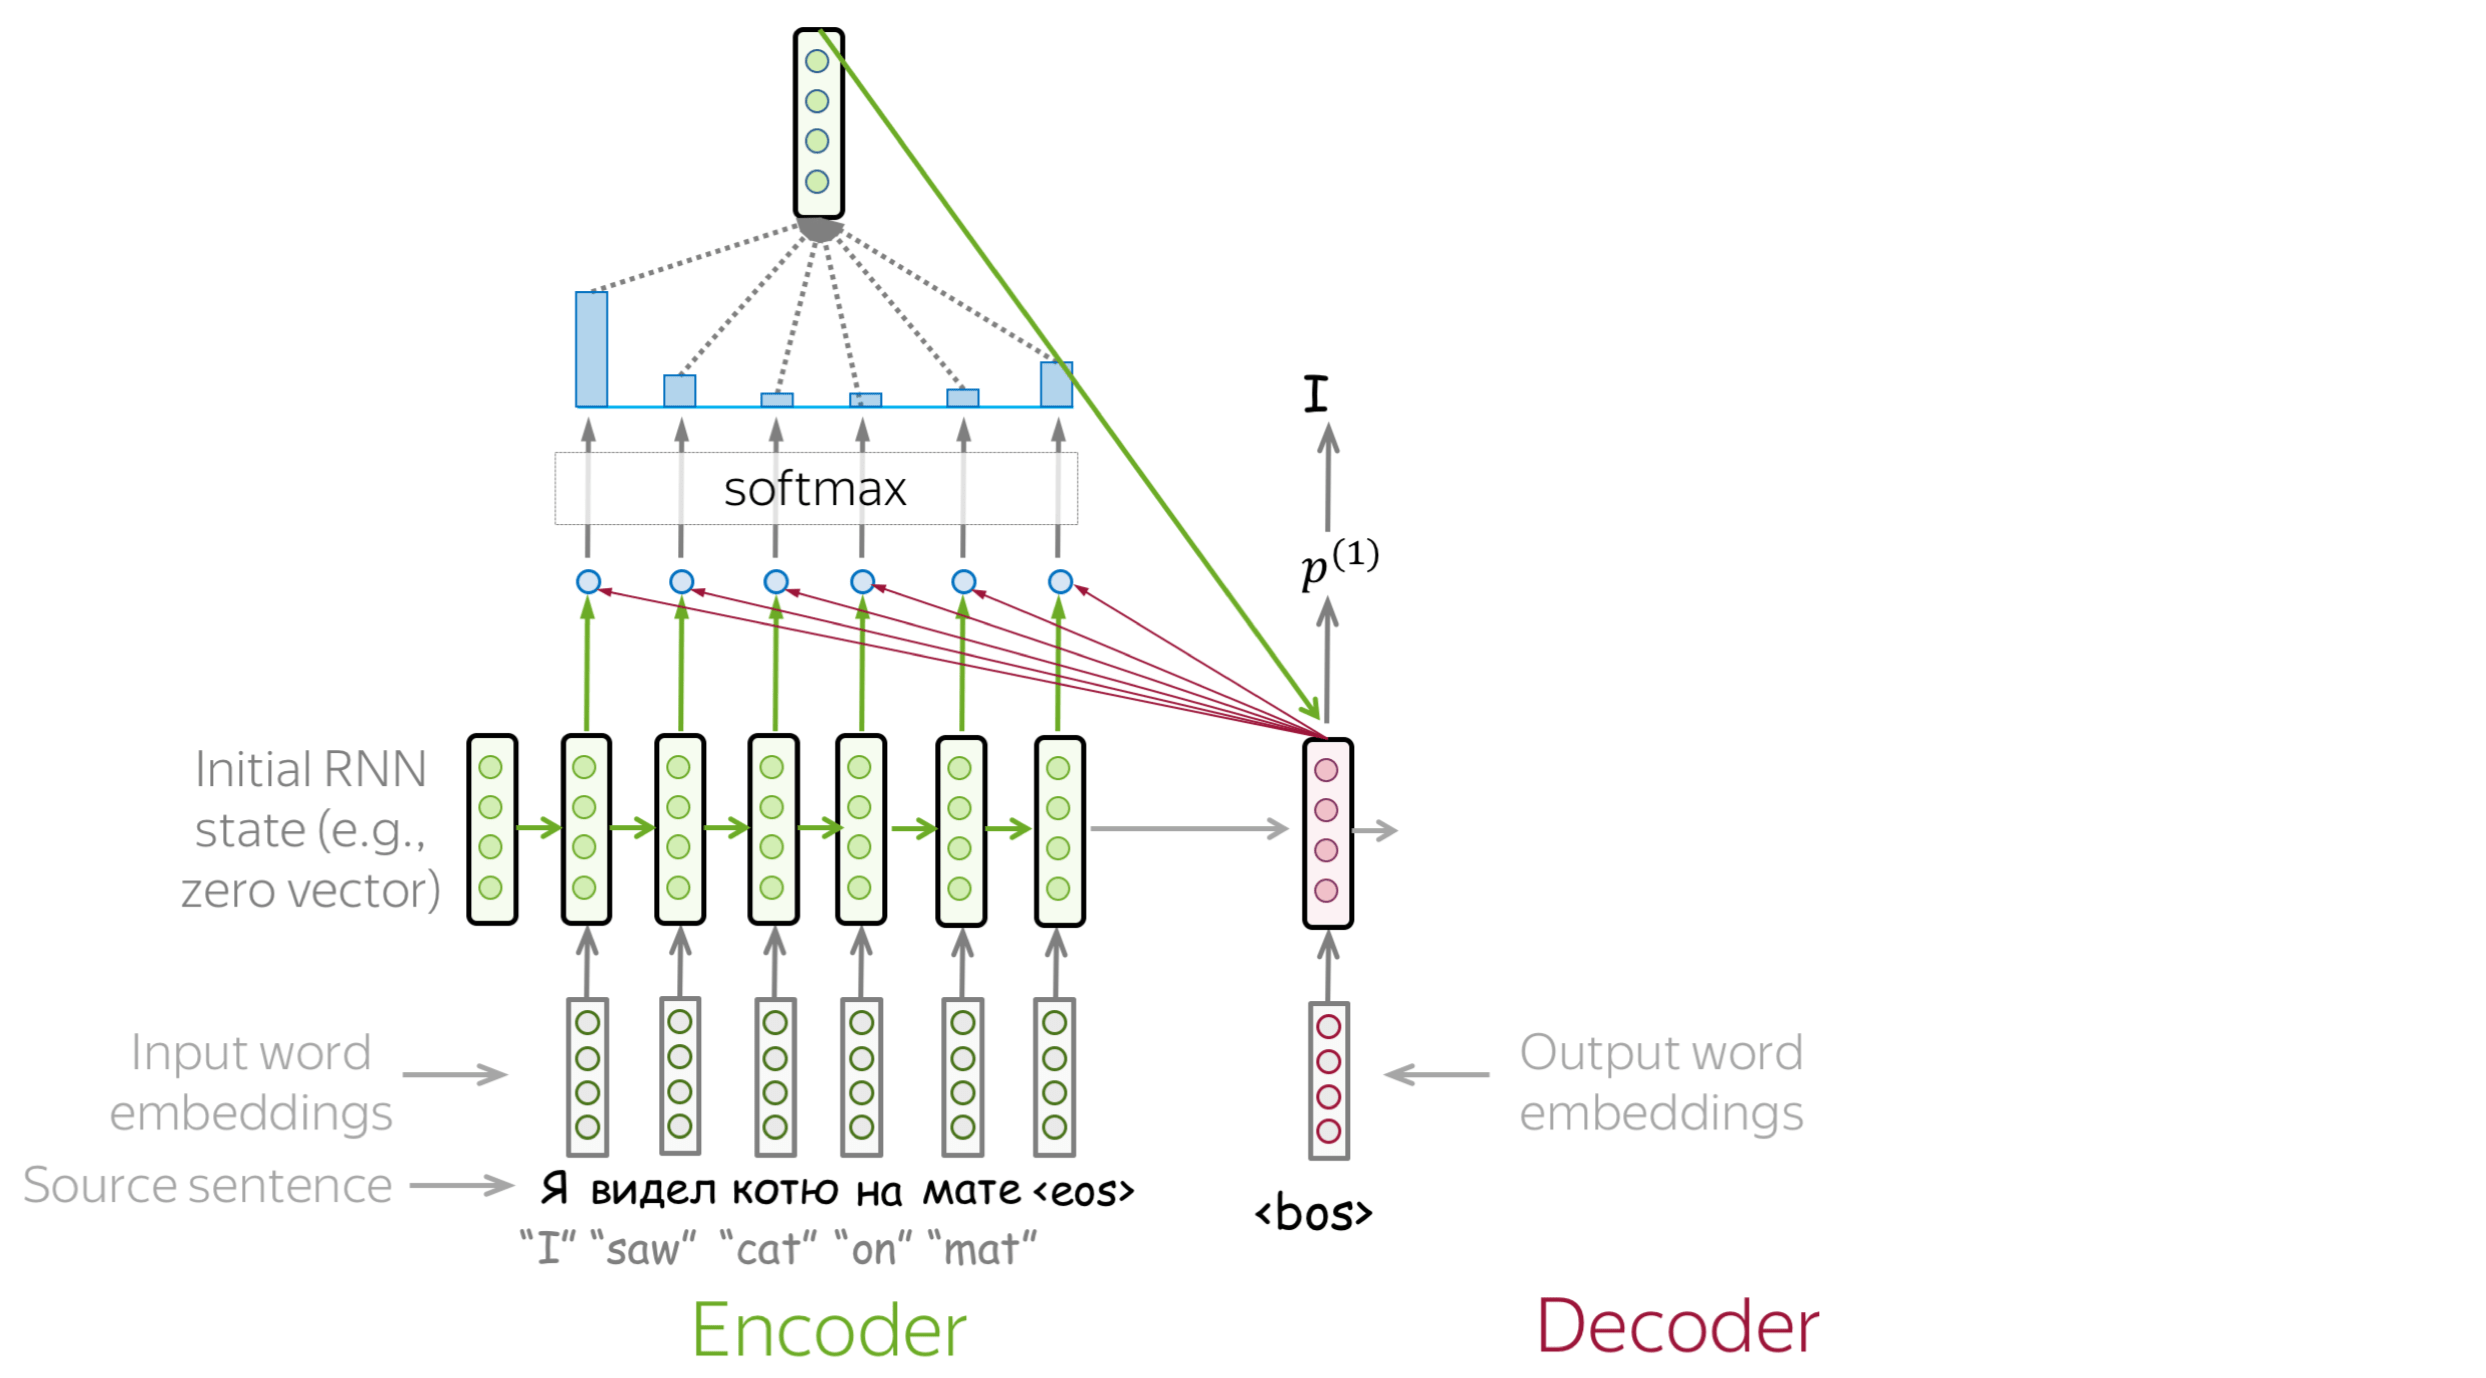
\includegraphics[width=1.0\textwidth]{images/1-min.png}
        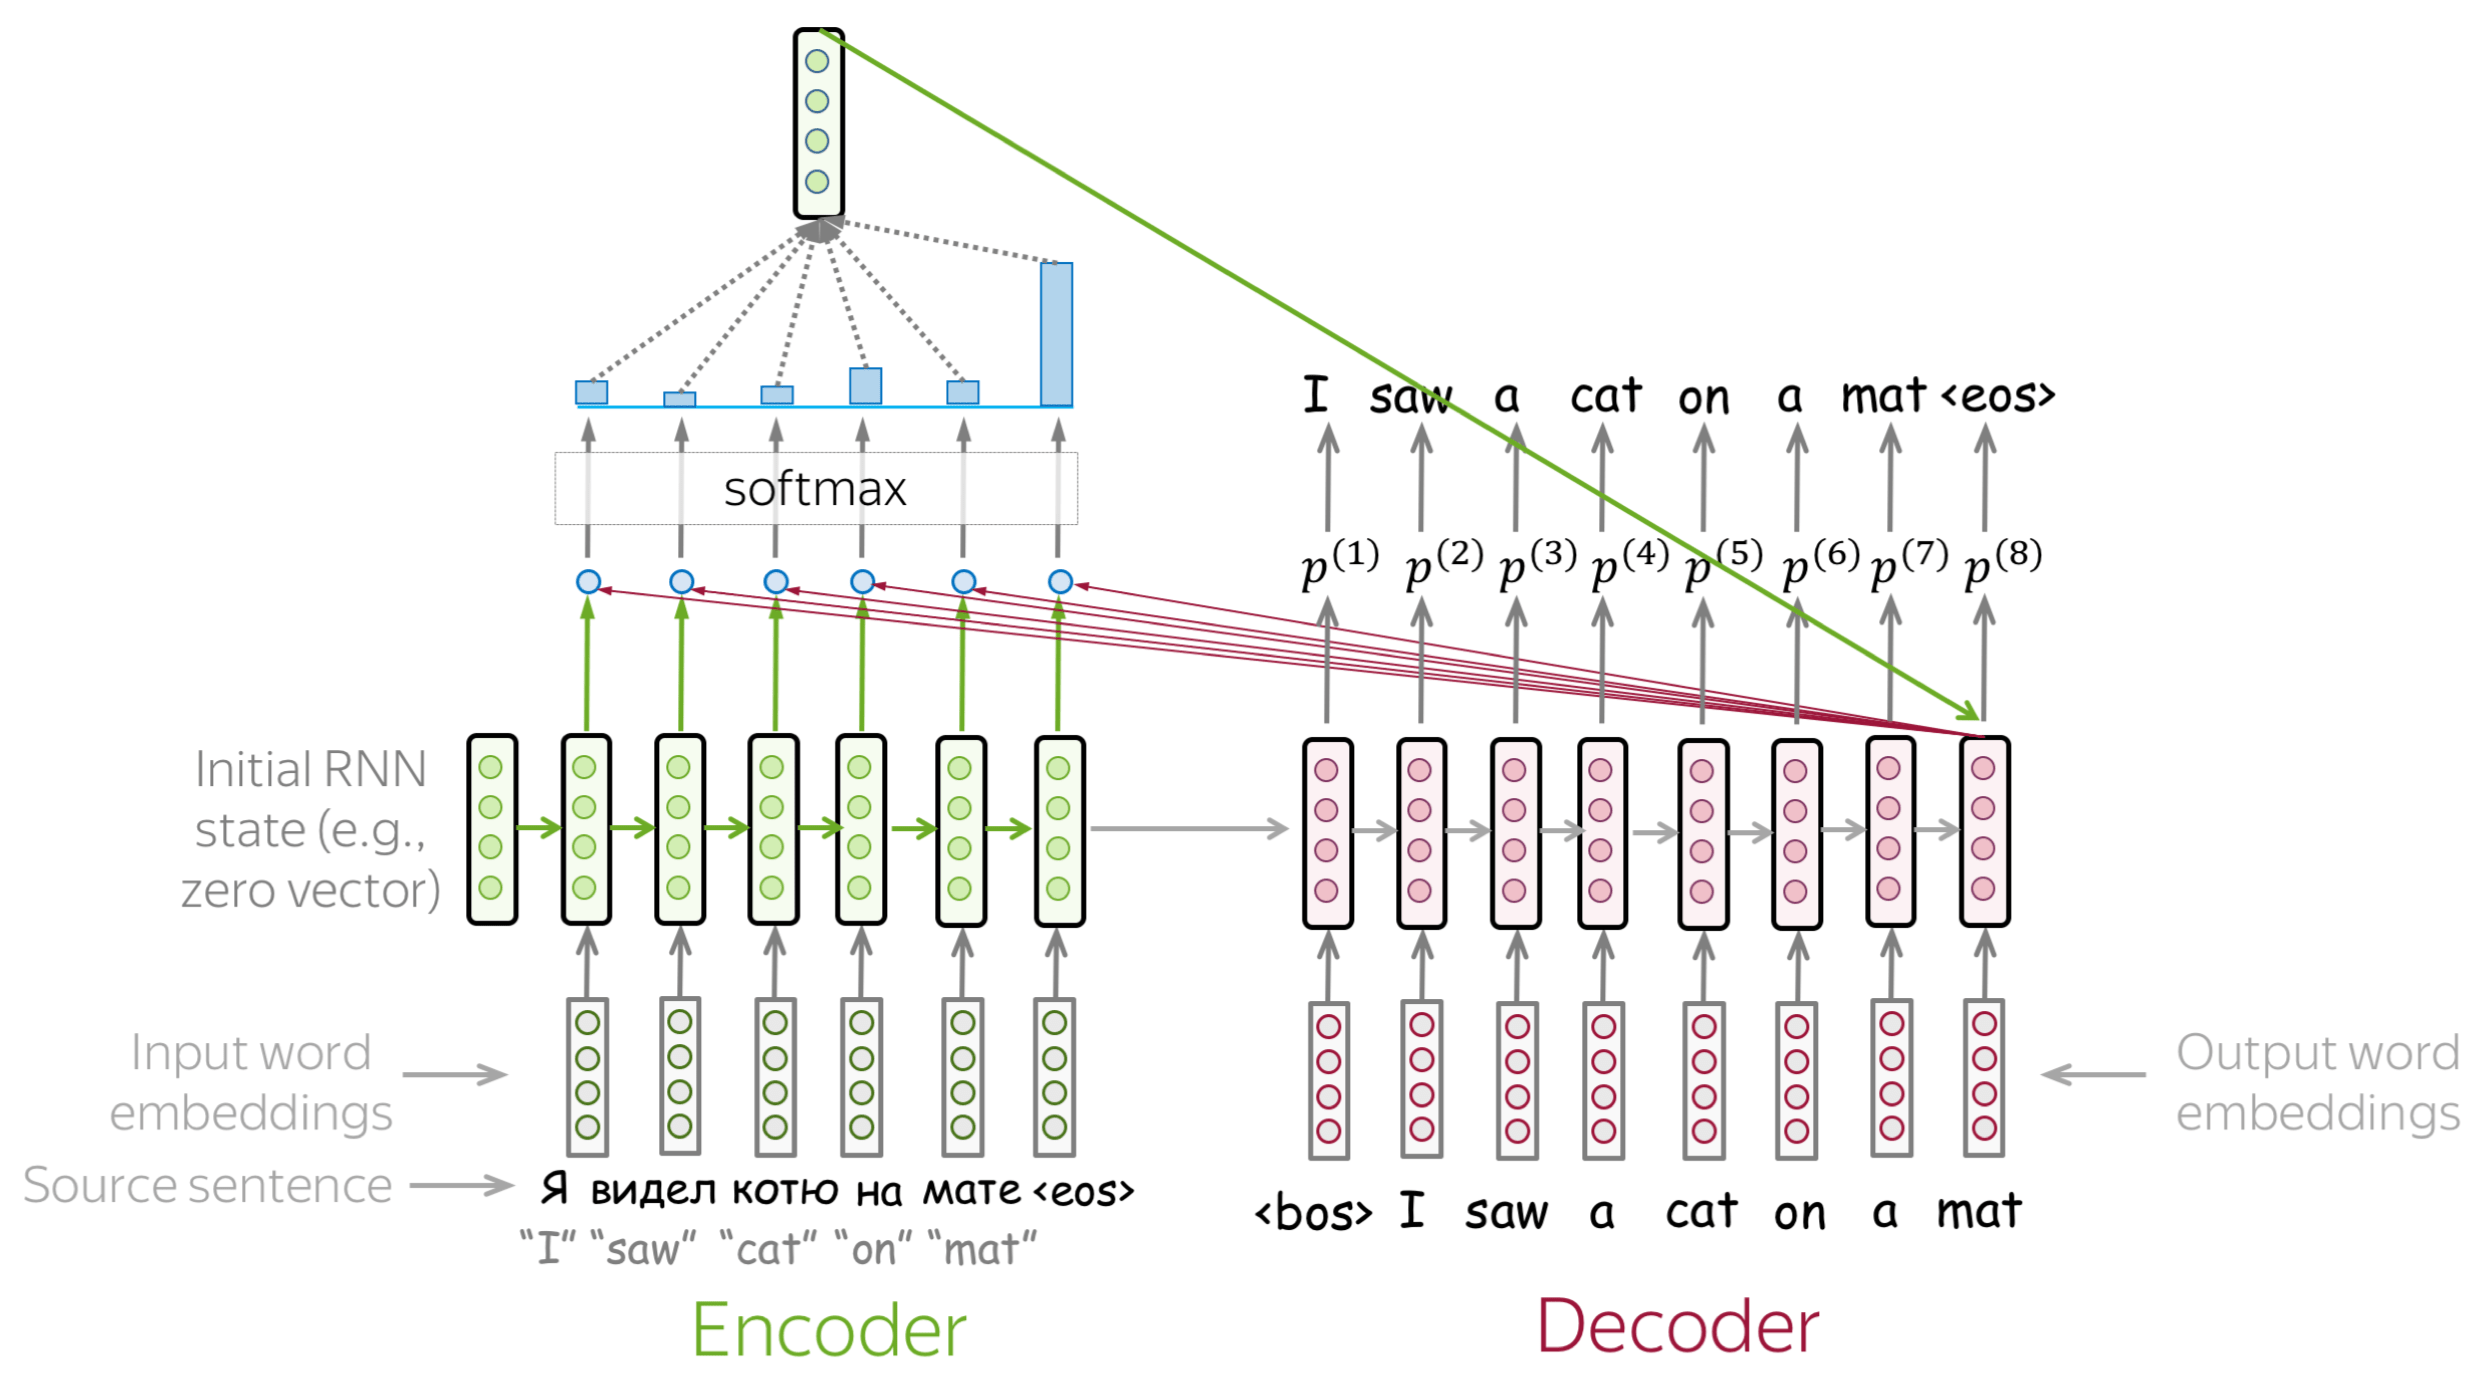
\includegraphics[width=1.0\textwidth]{images/8-min.png}
        \caption{Attention for machine translation where $Q$ is the hidden state of the decoder, $K$ and $V$ are the hidden states of the encoder.}
        \caption*{Image source: Lena Voita's blog}
\end{figure}
% 如果你研究过attention的数值细节,你会发现,attention的本质就是一个similarity measure。
% 它通过计算相似度,基于相似度来决定权重,也就是如何分配attention。
If you have studied the numerical details of Attention Mechanism, you will find that the essence of attention is a similarity measure.
It calculates the similarity, based on which it determines the weight, that is, how to allocate attention.
\section{Self-attention}
Self-attention is a special type of attention, where $Q = K = V$. 

\section{Multi-head Attention and Transformer model}
Multi-head attention is a mechanism that allows the model to focus on different parts of the sequence.
You can simply think it as a PLUS version of attention mechanism, it has many parallel attention mechanisms, and then concatenate the results.

\begin{figure}[H]
        \centering
        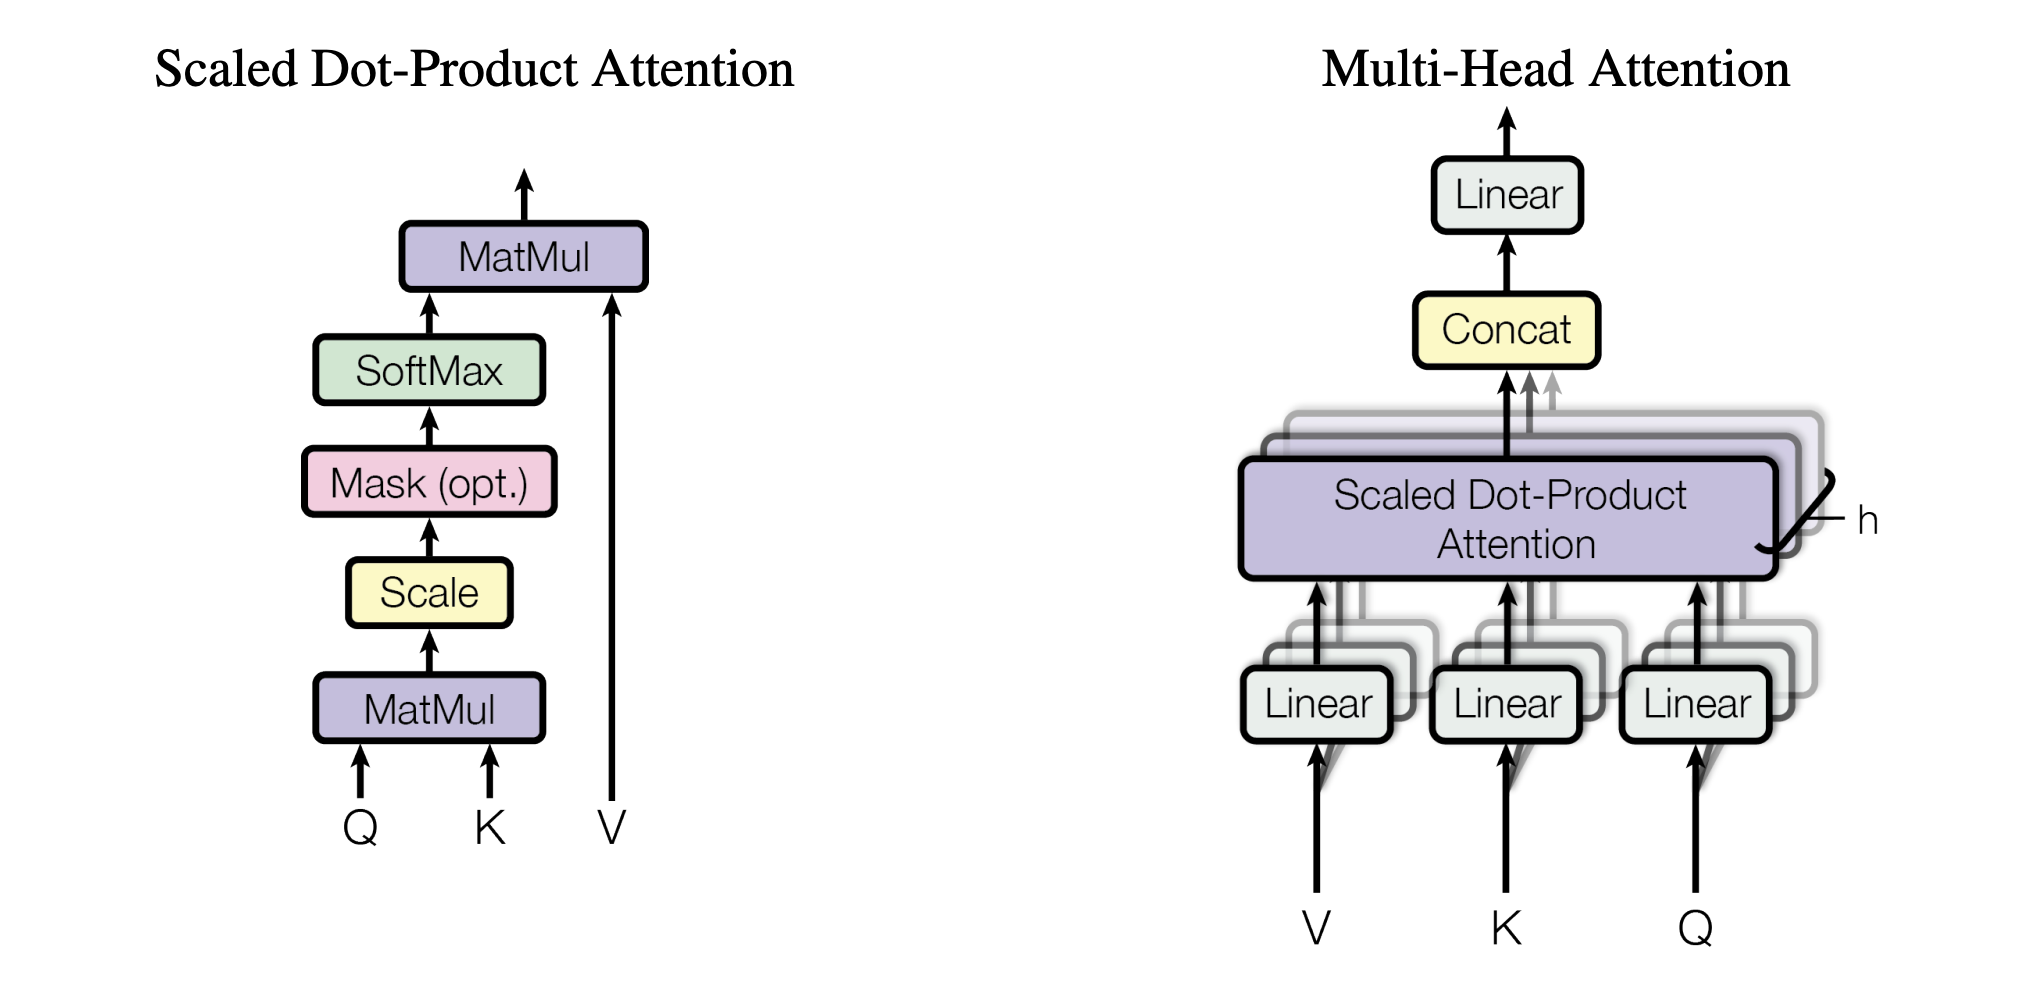
\includegraphics[width=0.8\textwidth]{images/multi-head attention.png}
        \caption{Multi-head attention}
        \caption*{Image source: PAPER Attention is all you need}
\end{figure}
\begin{figure}[H]
        \centering
        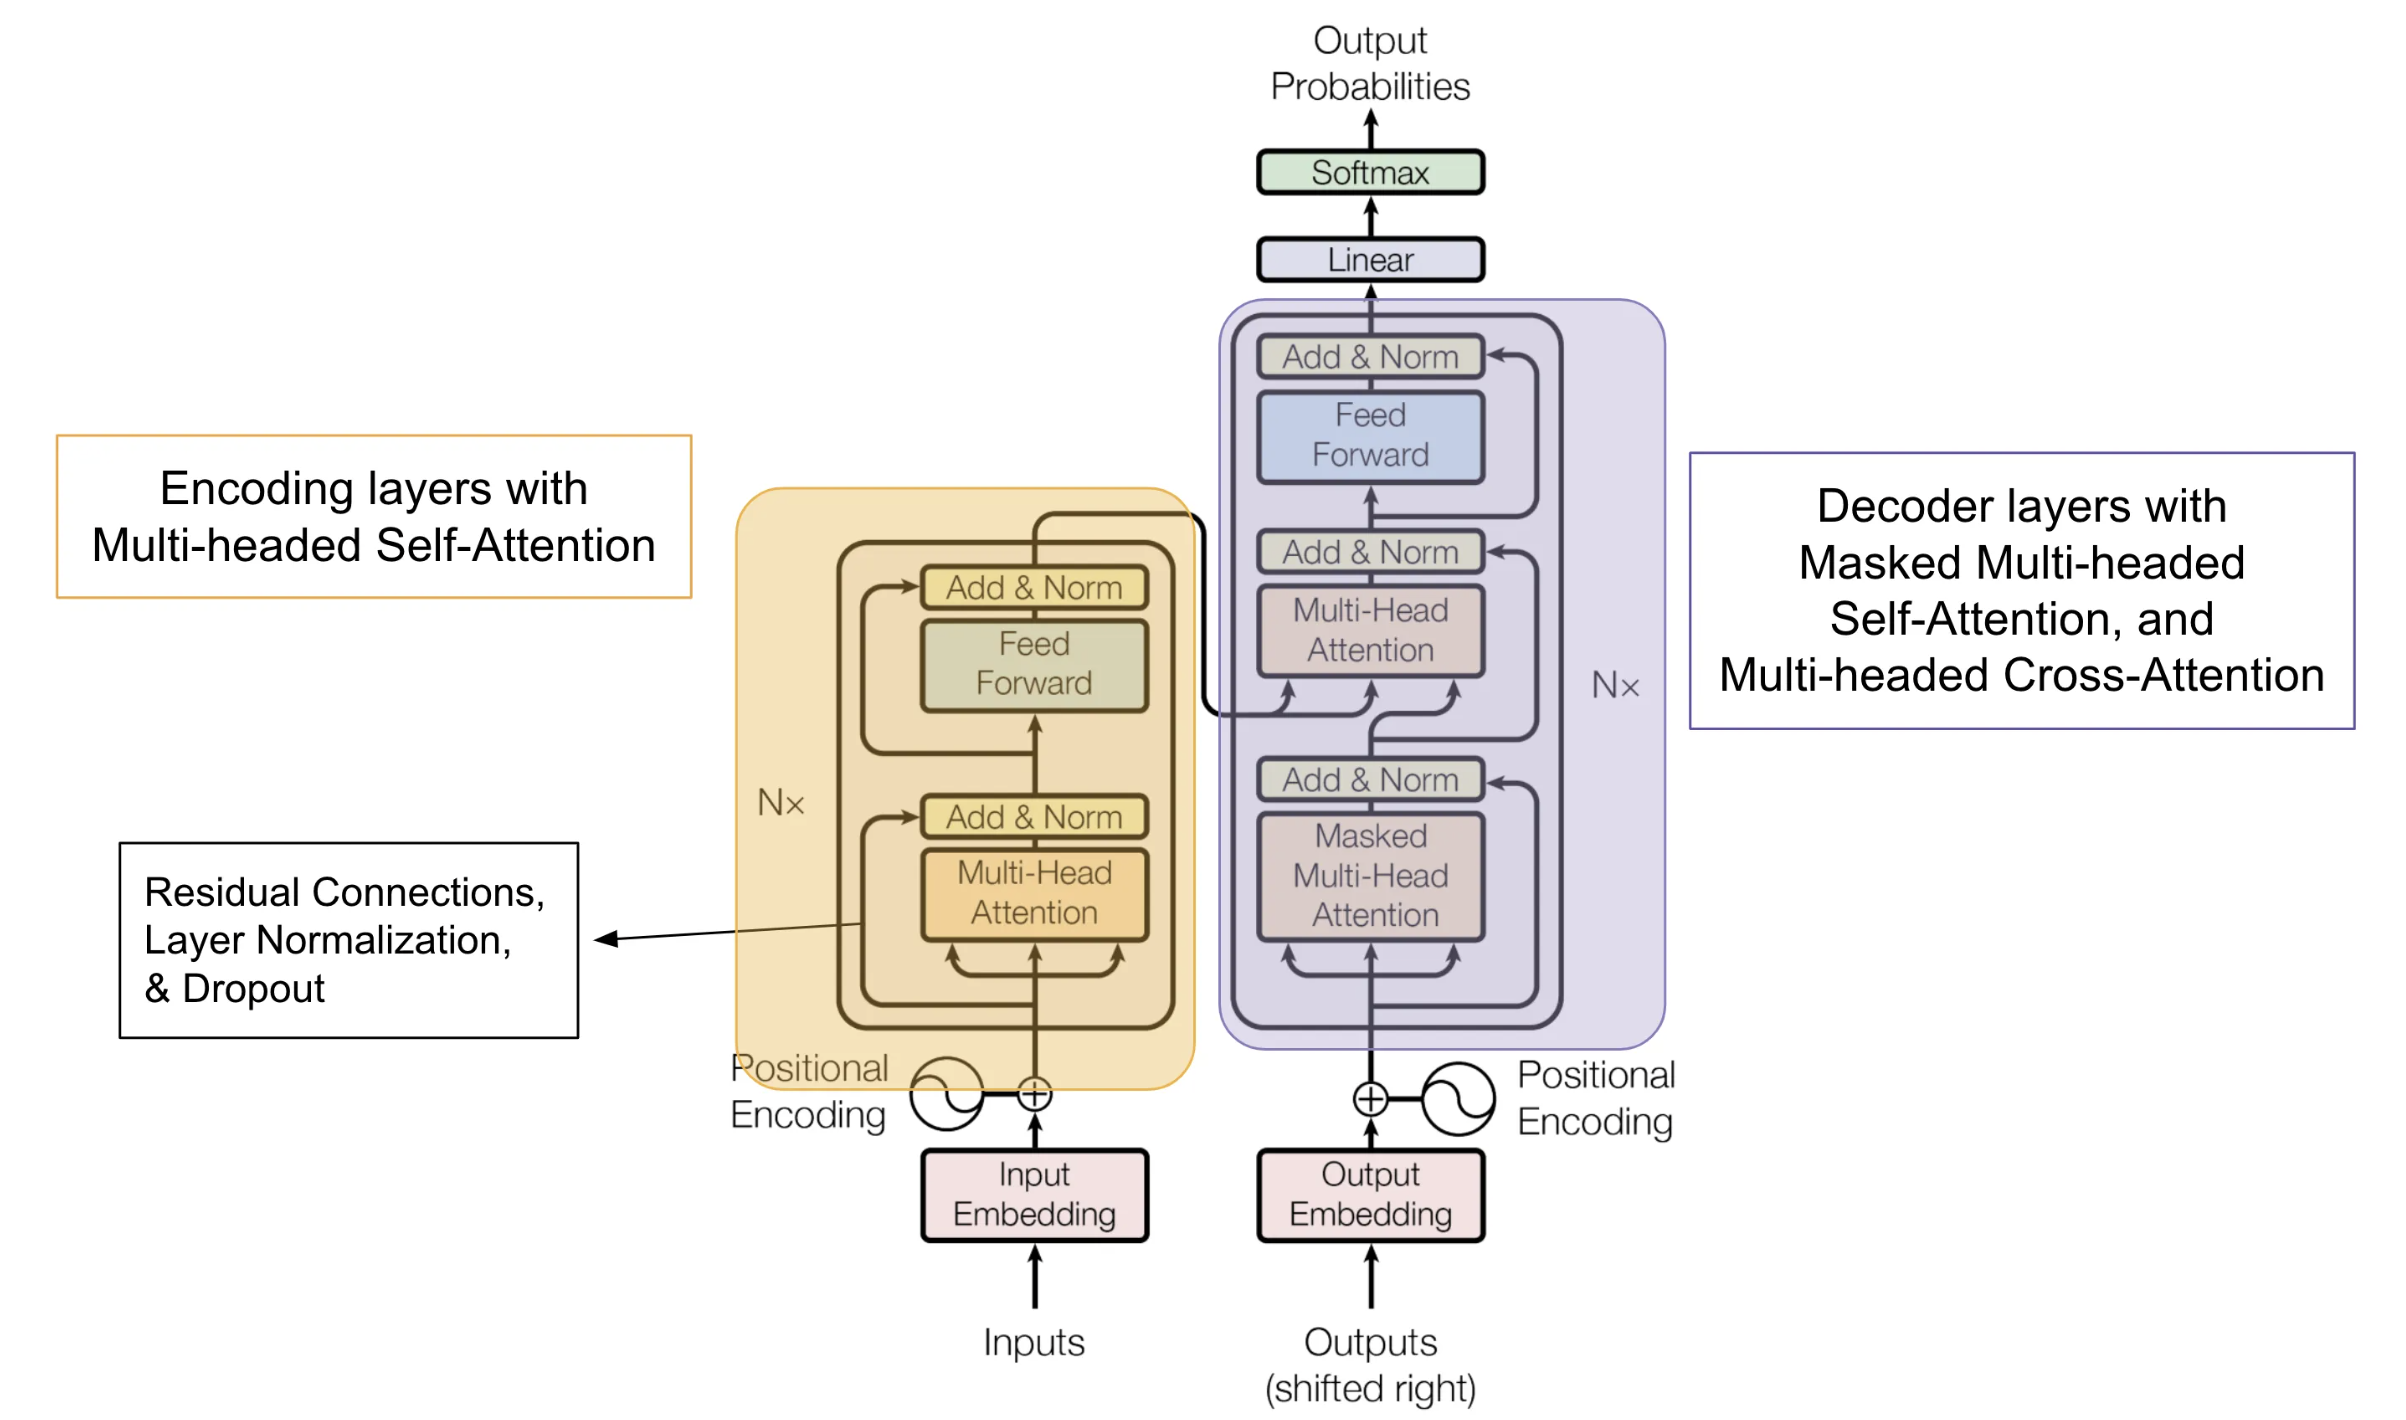
\includegraphics[width=1.0\textwidth]{images/transformer.png}
        \caption{Transformer}
        \caption*{Image source: PAPER Attention is all you need}
\end{figure}

\textbf{I think the core of the Transformer model is the attention mechanism.}
\section{Vision Transformer}
% 在过去几年,图像处理领域一般是用CNN,而文字处理领域是Attention。
In the past few years, CNN was generally used in image processing, while attention was used in text processing.
% 后来由于ChatGPT的出现,transformer based model在NLP领域取得了很大的成功,所以人们开始尝试把transformer应用到图像处理领域。
Later, due to the emergence of ChatGPT, transformer-based models achieved great success in the NLP field, so people began to try to apply transformers to image processing.
% 本质上,神经网络是一种universal function approximator,只要你的网络足够深,足够宽,你就可以拟合任何函数。
\textbf{Essentially, a neural network is a universal function approximator. As long as your network is deep enough and wide enough, you can fit any function.}
% 我并不奇怪transformer可以应用到图像处理领域,因为不管是文字还是图像,最后都是要转换成一个向量,然后再做一些操作。
I am not surprised that transformers can be applied to image processing because whether it is text or image, it needs to be converted into a vector in the end, and then some operations are performed.
% 我尝试过使用vision transformer来做一些图像处理的任务,效果和CNN差不多,这是我意料之外的。我期待的是vision transformer可以取得更好的效果,因为vision transformer的参数更多,performance 应该更好一点。
I have tried to use the vision transformer to do some image processing tasks, and the performance is similar to CNN, which is unexpected. 
What I expected was that the vision transformer could achieve better results because the vision transformer has more parameters, and the performance should be better.
% 也许他们的效果差不多是因为extract features的方式都是类似的,the way they calculate similarity is the same, dot product.
\textbf{\textcolor{blue}{Maybe their performance is similar because the way they extract features is similar, and the way they calculate similarity is the same, \textcolor{red}{dot product}.}}
Again, it is just a personal note. 
\section{Conclusion}
% 计算相似度/距离的方式有很多种,比如P-Norm similarity,Cosine similarity,Dot product similarity等等,你甚至还可以自己定义一些相似度的计算方式。
There are many ways to calculate similarity/distance, such as P-Norm similarity, Cosine similarity, Dot product similarity, etc., and you can even define some similarity calculation methods yourself.
% 不管是目标检测、图像分类、文本分类、推荐系统,相似度计算都是一个很重要的环节,因为如果model抓不住事物的特征的话,其他都搞不起来。
% 如何抓住一个东西的特征,也就是知道什么和什么是相似的,什么和什么是不相似的。
Whether it is object detection, image classification, text classification, or recommendation systems, similarity calculation is a very important link because if the model cannot grasp the characteristics of things, nothing else can be done.
\textbf{\textcolor{blue}{How to grasp the characteristics of something, that is, to know what is similar to what, and what is dissimilar to what.}} 
In my opinion, CNN, DNN, Attention, and Transformer are using the same similarity measure, which is the \textcolor{red}{dot product}. Again, it is just a personal note. 

\end{document}